\documentclass[12pt, a4paper]{report}

% all the other includes etc. are done in the thesis.sty file.
\usepackage{thesis}
\usepackage{ifthen}
\usepackage{datetime}

\renewcommand{\dateseparator}{-} % The ISO standard uses hyphens


% PDF Metadata
\newcommand{\authorName}{Mohamed Mahdi BEN SLIMA}
\newcommand{\doctitle}{Automatisation des infrastructures et des déploiements applicatifs}
\newcommand{\keywords}{IAC , GitOops , DevOps, Terraform, Ansible, Gitlab CI/CD, Kubernetes}

\hypersetup
{
    pdfauthor={\authorName},
    pdfsubject={\doctitle},
    pdfkeywords={\keywords}
}

% begin document
\begin{document}
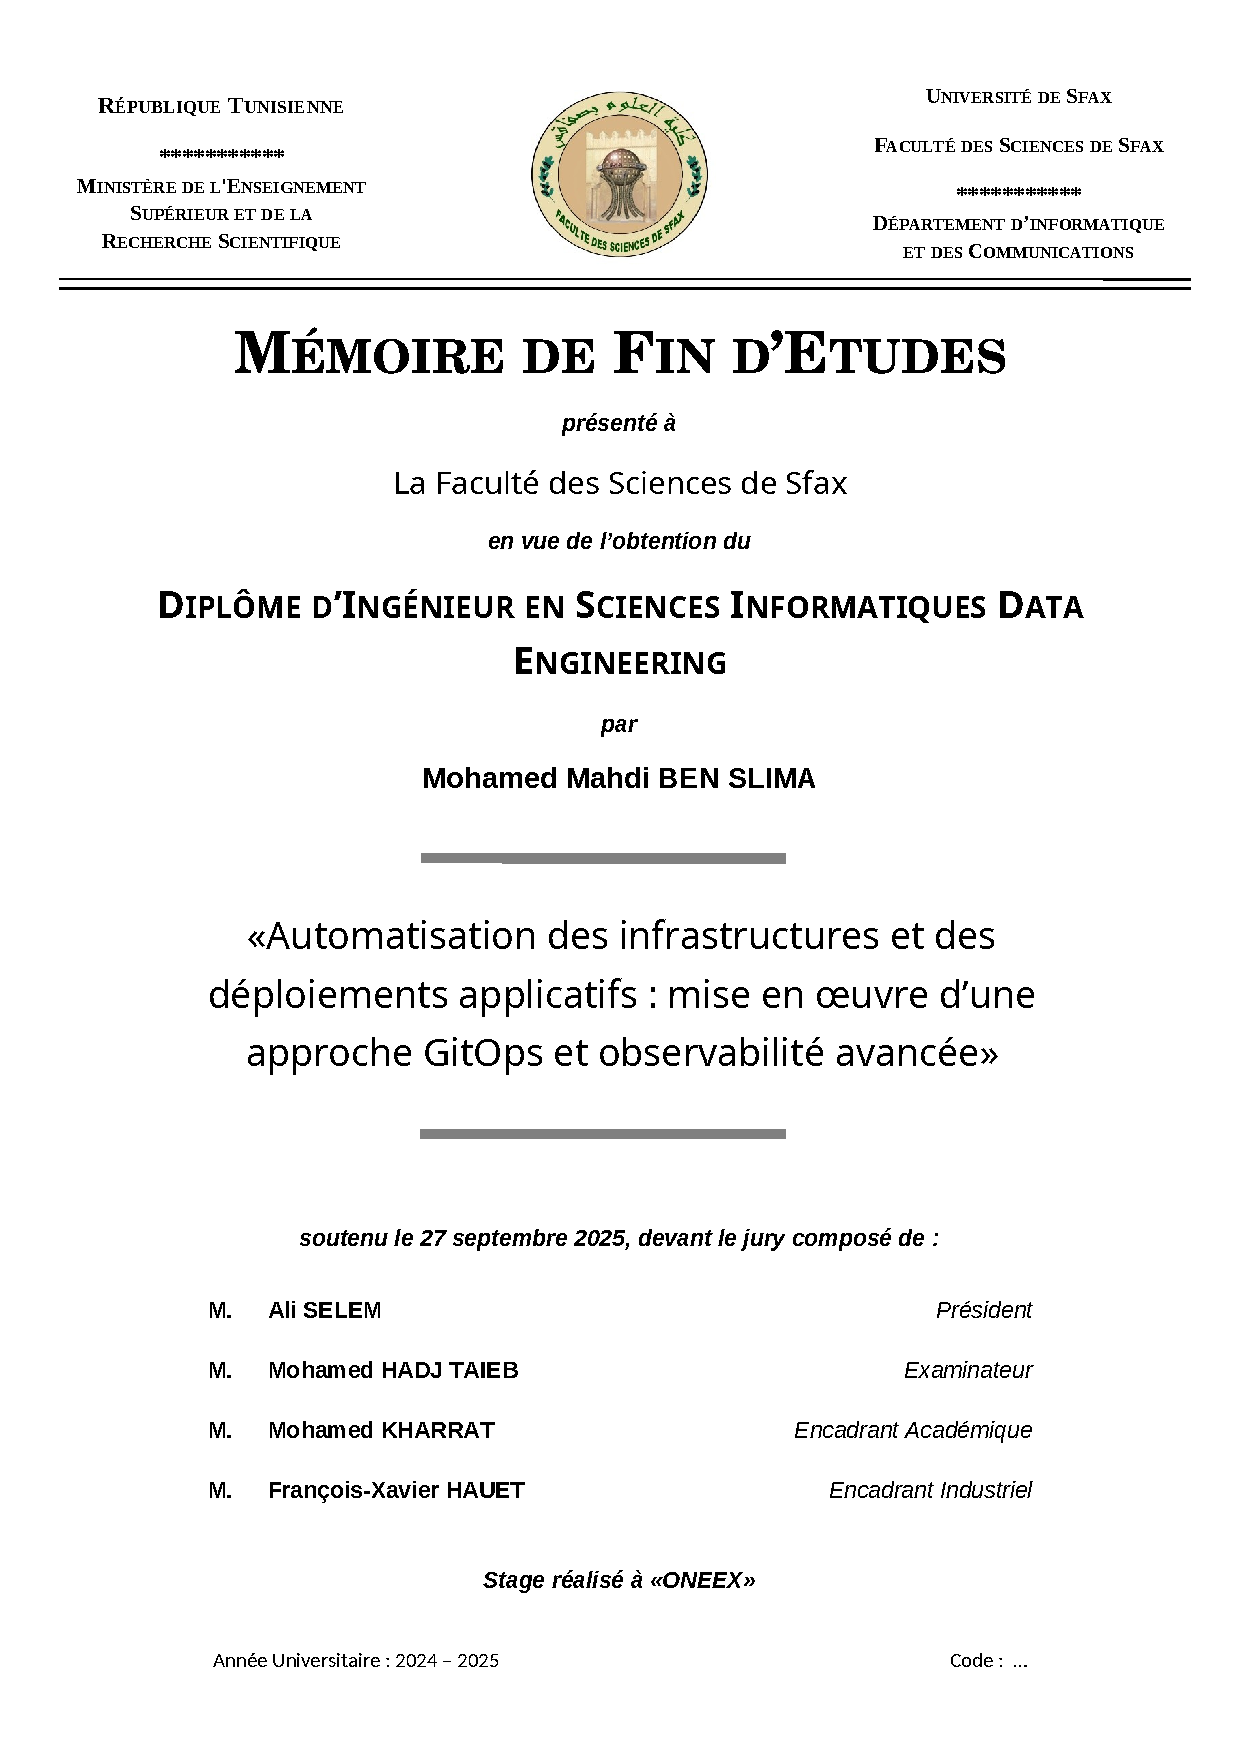
\includepdf[pages=-]{page de garde.pdf}
\renewcommand{\headrulewidth}{0pt}

% misc
%% PAGE DE TITRE EN FRANÇAIS

\begin{titlepage}
	\headheight = 0pt

		{%
			\fontsize{9pt}{9pt}\selectfont%
			\renewcommand\arraystretch{2}

			\begin{longtable*}{p{0.3\textwidth} p{0.1\textwidth} p{0.1\textwidth} p{0.3\textwidth}}
				\centering République Tunisienne\\
				Ministère de l'Enseignement Supérieur et de la Recherche Scientifique%
				& \centering \makebox[\linewidth][c]{
\includegraphics[width=0.15\textwidth]{figures/favicon-white.png}}
				& \centering \makebox[\linewidth][c]{
\includegraphics[width=0.15\textwidth]{figures/logo_fss.png}}
				& \centering \department\\ \tabularnewline
				\centering Université de Sfax\\
				Faculté des Sciences de Sfax%
				& & &
				\centering \textbf{\doctype}\\
				\degree~en~\major%
				\tabularnewline
			\end{longtable*}
		}

	\vspace*{8pt}

	\begin{center}

		{
			\fontsize{33pt}{33pt}\selectfont%
			\textsc{\textbf{\doctype}}\\%
		}

		\vspace*{14pt}
		\textit{Présenté à}\\%

		\vspace*{3pt}
		La Faculté des Sciences de Sfax\\%
		\department\\%

		\vspace*{14pt}
		\textit{En vue de l'obtention du diplôme de}\\%

		\vspace*{3pt}
		\textsc{\degree~en~\major}\\%

		\vspace*{14pt}
		\textit{Par}\\%

		\vspace*{3pt}
		\begin{large}
			\textbf{\authorName}\\%
		\end{large}

		\vspace*{25pt} {
			\begin{spacing}{0.05}
				\rule{300pt}{2pt}\\
				\rule{300pt}{0.75pt}\\
			\end{spacing}
			\vspace{20pt}
			\begin{spacing}{0.9}
				\fontsize{26pt}{26pt}\selectfont%
				\textsc{\textbf{\doctitle}}\\%
			\end{spacing}
			\vspace{5pt}
			\begin{spacing}{0.05}
				\rule{300pt}{0.75pt}\\
				\rule{300pt}{2pt}\\
			\end{spacing}
		}

		\vfill
		\begin{longtable*}{ p{0.5\textwidth} p{0.2\textwidth} }
			\president & Président du jury
			\tabularnewline\reviewer & Rapporteur
			\ifthenelse{\equal{\secondReviewer}{M. Nom du second rapporteur}}{}{%
				\tabularnewline\secondReviewer & Rapporteur}
			\ifthenelse{\equal{\thirdReviewer}{M. Nom du troisième rapporteur}}{}{%
				\tabularnewline\thirdReviewer & Rapporteur}
			\tabularnewline\supervisor & Directeur de mémoire
			\ifthenelse{\equal{\cosupervisor}{M. Nom du co-directeur}}{}{%
				\tabularnewline\cosupervisor & Co-directeur de mémoire}
			\tabularnewline
		\end{longtable*}

		\vspace*{3pt}
		\defenseDate

	\end{center}
\end{titlepage}


\setcounter{page}{0}
\pagenumbering{roman}   %from here on, start the 'real' page numbering, from 1, with normal digits
\renewcommand{\thepage}{\Roman{page}}
\normalsize

% \chapter*{\centerline{Dédicace}}\label{chapter:dedication}
% \textbf{Je dédie ce travail à :}

\medskip

\textbf{Mes chers parents, Neji et Imen}
Je ne trouverai jamais les mots justes pour vous exprimer toute ma reconnaissance. Sans vos sacrifices, vos prières et votre amour inconditionnel, je n’aurais jamais pu arriver jusqu’ici. Je vous souhaite une longue vie remplie de santé, de paix et de bonheur.

\medskip

\textbf{Mon cher frère, Haythem}
Que ce travail soit l’occasion de te témoigner toute ma gratitude pour ta présence constante, ton soutien indéfectible et la confiance que tu m’as accordée. Ton appui m’a donné la force de surmonter chaque obstacle. Je te souhaite, à mon tour, beaucoup de réussite dans ta vie.

\medskip

\textbf{Tous les membres de ma famille}
Merci pour votre amour, vos encouragements et votre bienveillance. Chacun de vous, à sa manière, a contribué à ce parcours.

\medskip

\textbf{Tous mes amis}
Merci pour votre présence sincère et votre amitié fidèle, qui m’ont soutenu dans les moments difficiles.

\medskip

\textbf{À vous tous}
Je vous dédie ce travail avec toute ma gratitude et mon affection.
% \pagebreak

% \chapter*{\centerline{Remerciements}}\label{chapter:acknowledgments}
% [YOUR TEXT GOES HERE]
% \pagebreak

\chapter*{\centerline{Résumé}}\label{chapter:abstract}
Face à l’essor des architectures distribuées et aux exigences croissantes en matière de sécurité, de fiabilité et de conformité, les infrastructures classiques montrent rapidement leurs limites. Ce projet s’est attaché à repenser en profondeur la manière de concevoir et d’opérer une infrastructure informatique, dans un contexte réel au sein de l’entreprise Oneex.

L’approche adoptée ne s’est pas limitée à automatiser des déploiements ou à enchaîner des outils DevOps. Il s’est agi de construire une plateforme cohérente, robuste et évolutive, capable d’orchestrer des services critiques, de protéger les secrets, de tracer chaque changement et d’alerter intelligemment en cas d’incident.

Le système mis en place s’appuie sur une chaîne complète — de l’infrastructure virtuelle à la supervision applicative — avec un enchaînement réfléchi d’outils tels que Proxmox, Terraform, Ansible, Kubernetes, Vault, Argo CD et la stack d’observabilité Prometheus / Grafana / Loki / Tempo. Ces choix ne sont pas dictés par la mode, mais par leur complémentarité, leur adaptabilité et leur capacité à s’inscrire dans une démarche GitOps sécurisée.

Au-delà des aspects techniques, ce projet a permis d’explorer les vraies conditions de l’industrialisation : homogénéité entre environnements, résilience face aux erreurs humaines, visibilité sur les flux, et gouvernance des accès. Il constitue une base solide pour porter la transformation numérique de l’infrastructure de Oneex vers un modèle plus agile, contrôlé et résilient.
\pagebreak

\chapter*{\centerline{Liste des abréviations et des termes}}\label{chapter:terms}
\begin{longtable*}{p{3cm}p{10cm}}
	FSS & Faculty of Sciences of Sfax \\
	OTel & OpenTelemetry \\
	% more entries...
\end{longtable*}

\pagebreak

\phantomsection
\setcounter{tocdepth}{2}
\renewcommand{\contentsname}{Table des matières}
\tableofcontents

\clearpage \phantomsection
\renewcommand{\listfigurename}{Liste des figures}
\setcounter{figure}{0}
\addcontentsline{toc}{chapter}{\listfigurename}
\listoffigures

\clearpage \phantomsection
\renewcommand{\listtablename}{Liste des tableaux}
\addcontentsline{toc}{chapter}{\listtablename}
\listoftables

% chapters
\cleardoublepage
\pagenumbering{arabic}
\setcounter{page}{1}
% chapters
\chapter{Introduction générale}
\section{Introduction}

Dans un contexte technologique en constante évolution, marqué par une forte concurrence et une accélération des cycles de développement, l’importance des concepts que nous avons mis en œuvre est devenue capitale. L’automatisation, qui était autrefois perçue comme un avantage optionnel, s’impose désormais comme une nécessité incontournable pour garantir la fiabilité, la sécurité et la rapidité des processus.

\section{Présentation de l'organisme d'accueil}

Oneex est une entreprise française basée à Clermont-Ferrand, avec un établissement secondaire à Paris. Elle est spécialisée dans la conception et le développement de solutions logicielles et matérielles dédiées à la vérification d’identité et à l’analyse documentaire. Grâce à des technologies avancées telles que l’intelligence artificielle et des capteurs avancés tel que les lecteurs NFC , infrarouge , hyper resolution pour une analyse approfondie des documents , qui n'est autrement pas possible a l'oeil nu, Oneex propose des solutions innovantes pour lutter contre la fraude documentaire.

\subsection{Historique de l’entreprise}

\begin{itemize}
	\item \textbf{Création de la société (2017)}
	      Le concept Oneex est né de l’initiative de son fondateur, confronté à la problématique de l’analyse des documents d’identité. N’ayant trouvé aucune solution souveraine respectant les contraintes réglementaires sur les données personnelles, il a décidé de créer et de développer Oneex.

	\item \textbf{Recherche et développement (2018-2020)}
	      Pendant deux années, l’entreprise s’est consacrée à la recherche et au développement. Le logiciel ScanApp a ainsi été créé pour reproduire la vision humaine grâce à une intelligence artificielle capable d’analyser avec précision le pays, le format et les spécificités techniques d’un document.

	\item \textbf{Déploiement de la solution Desktop (2020)}
	      Forte de ce développement, Oneex a lancé une offre complète associant hardware et software, donnant naissance à la solution Desktop.

	\item \textbf{Reconnaissance et impact (2021-2023)}
	      L’entreprise a rapidement acquis une reconnaissance dans son domaine, obtenant des distinctions et certifications de la part de leaders de l’industrie. Elle poursuit aujourd’hui sa croissance à l’international.

	\item \textbf{Percées technologiques et évolution (2023-2024)}
	      Oneex a enrichi ses produits de nouvelles fonctionnalités, notamment le monitoring à distance, l’accès à des statistiques détaillées, la gestion autonome du parc matériel et un accompagnement expert en fraude documentaire. Après une levée de fonds importante en 2024, l’entreprise développe de nouveaux produits pour renforcer son positionnement en tant que leader de l’analyse documentaire.
\end{itemize}

% En 2025, François-Xavier Hauet, mon tuteur de stage, a rejoint l’entreprise en tant que Directeur Général. Fort d’une carrière de haut fonctionnaire et d’une expertise reconnue dans la transformation numérique, notamment à la Présidence de la République, il apporte à Oneex une vision stratégique et opérationnelle précieuse. Sous son impulsion, l’entreprise engage le développement de la nouvelle génération de ses solutions.

\subsection{Domaine d'activité}

A travers ses systemes de detection de faux documents , capables a operer en mode online ainsi qu'offline Oneex propose des solutions transversales adaptées à de nombreux secteurs, notamment la santé, les banques, la sécurité et le contrôle d’accès, la location de véhicules, ainsi que les aéroports et compagnies aériennes.

\subsection{Organisation interne}

La direction et les équipes de Oneex rassemblent des profils pluridisciplinaires aux parcours variés :

\begin{description}
	\item[Alexandre Casagrande] Fondateur et Président Directeur Général. Après 12 ans au sein du Ministère des Armées et plusieurs années dans la sûreté de grands groupes, il a fondé Oneex avec la volonté de développer une solution souveraine et innovante.

	\item[François-Xavier Hauet] Directeur Général. Ancien haut fonctionnaire, il a piloté la transformation numérique du Centre Interministériel de Crise puis de la Présidence de la République avant de rejoindre Oneex en 2025.

	\item[Julien Otal] CTO. Développeur spécialisé dans le multiplateforme, il possède une solide expérience dans la sécurisation de systèmes critiques et la traçabilité des flux.

	\item[Xavier Matton] Directeur des Opérations. Ingénieur et ancien officier au Ministère de l’Intérieur, il est expert en contrôle des flux et lutte contre la fraude documentaire.

		%\item[Damien Lazardeux] Architecte Logiciels. Spécialiste des technologies .NET, il conçoit les systèmes logiciels de détection des faux papiers.

	\item[Sébastien Kowalczuk] Directeur des Opérations Sud-Ouest. Ancien enquêteur en contre-ingérence économique, il apporte une expertise forte en sécurité des données sensibles.
\end{description}

\begin{figure} [H]
	\centering
	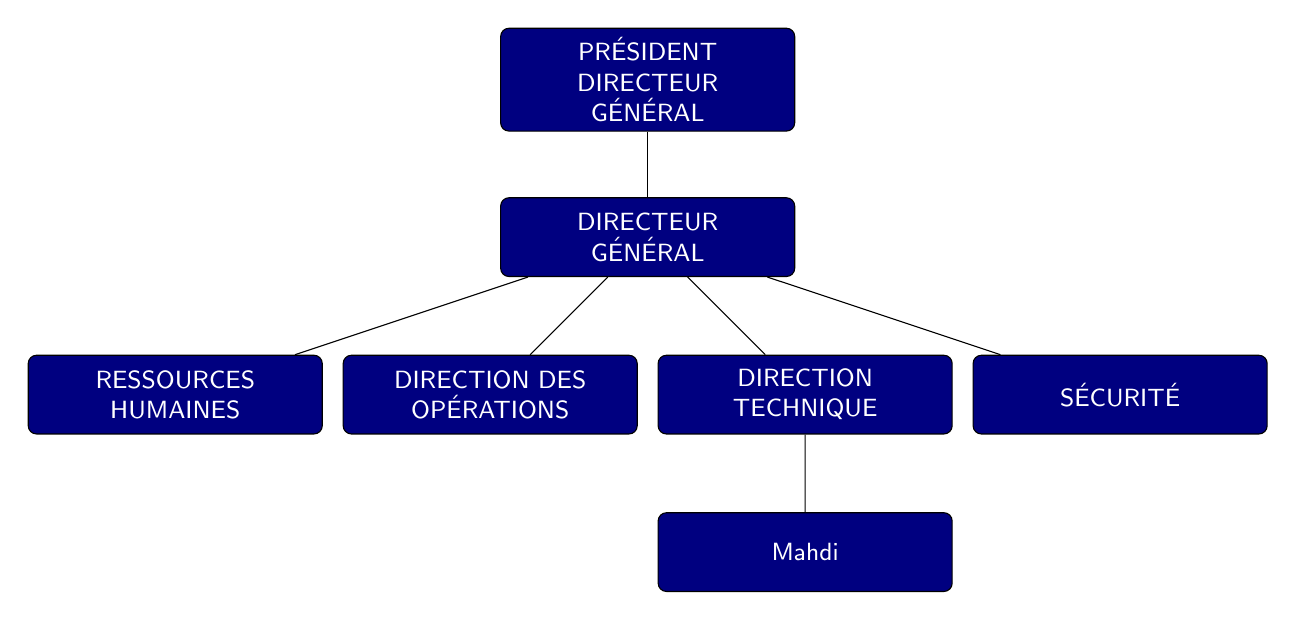
\begin{tikzpicture}[
			edge from parent/.style={draw, -},
			level 1/.style={sibling distance=60mm, level distance=20mm},
			level 2/.style={sibling distance=40mm, level distance=20mm},
			every node/.style={
					draw,
					fill=blue!50!black,
					rounded corners=3pt,
					text=white,
					align=center,
					font=\sffamily\small,
					text width=35mm,
					minimum height=10mm
				}
		]
		\node {PRÉSIDENT \\ DIRECTEUR \\ GÉNÉRAL}
		child {node {DIRECTEUR \\ GÉNÉRAL}
				child {node {RESSOURCES \\ HUMAINES}}
				child {node {DIRECTION DES \\ OPÉRATIONS}}
				child {node {DIRECTION \\ TECHNIQUE}
						child {node {Mahdi}}
					}
				child {node {SÉCURITÉ}}
			};
	\end{tikzpicture}
	\caption{\textit{Organisation interne simplifiée de l'entreprise}}
	\label{fig:organisation_interne}
\end{figure}

\subsection{Produits et services de l'entreprise}

Oneex propose une gamme de solutions matérielles et logicielles, parmi lesquelles trois produits phares :

\begin{itemize}
	\item \textbf{Oneex Desktop} : une station de vérification d’identité clé en main simple et intuitive pour un accueil sécurisé , cette derniere effectue chaque scan en toute confiance. Le desktop Oneex reconnaît instantanément tous les documents d'identité de 197 pays — garantissant une vérification sûre et précise à chaque fois.
	      \begin{figure} [H]
		      \centering
		      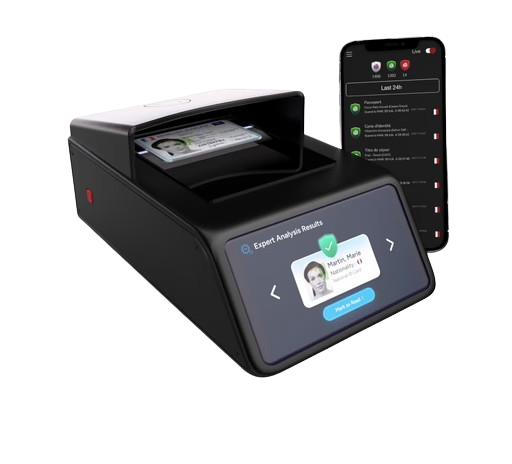
\includegraphics[width=.5\textwidth]{figures/Oneex desktop.png}
		      \caption{\textit{Oneex Desktop}}
		      \label{fig:Oneex desktop}
	      \end{figure}
	\item \textbf{Oneex Suitcase} : une valise mobile permettant de réaliser des contrôles sur le terrain , portable et robuste , elle laisse les utilisateurs se profiter d’un système mobile de vérification d’identité fiable et sécurisé.
	      \begin{figure} [H]
		      \centering
		      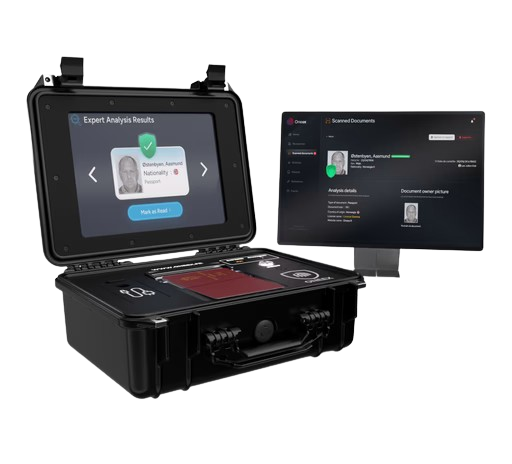
\includegraphics[width=.5\textwidth]{figures/Oneex suitcase.png}
		      \caption{\textit{Oneex Suitcase}}
		      \label{fig:Oneex Suitcase}
	      \end{figure}
	\item \textbf{Oneex Kiosk} : un kiosque en libre-service pour l’accueil et le contrôle des visiteurs. Permet Accueiller vos visiteurs sans assistance grâce à une vérification rapide et un accès direct.Une solution pensée pour vos opérations, combinant biométrie avancée et automatisation complète de l’accès visiteurs.
	      \begin{figure} [H]
		      \centering
		      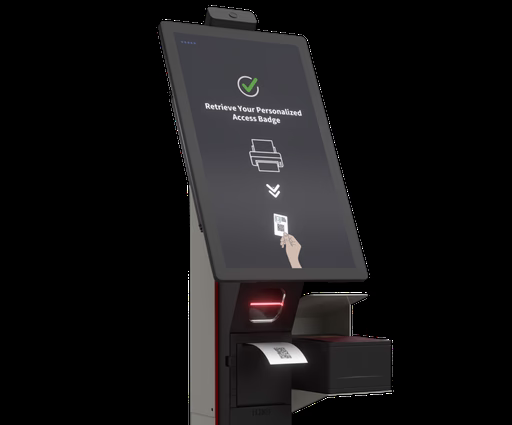
\includegraphics[width=.5\textwidth]{figures/Oneex kiosk.png}
		      \caption{\textit{Oneex Kiosk}}
		      \label{fig:Oneex Kiosk}
	      \end{figure}
\end{itemize}

Ces produits sont complétés par la suite logicielle Oneex Cloud et ScanApp, garantissant un pilotage centralisé et une intégration fluide dans les environnements clients.

Son application \emph{Oneex Cloud}, une plateforme offre un contrôle centralisé et un suivi avancé des vérifications d’identité.

Cette plateforme permet un :

\begin{itemize}
	\item \textbf{Suivi des documents scannés} : historique complet, résultats détaillés et traçabilité optimale.
	\item \textbf{Demande d’expertise} : sollicitation d’experts pour garantir des analyses approfondies et fiables.
	\item \textbf{Statistiques avancées} : exploitation des tendances de la fraude pour optimiser la gestion des incidents.
\end{itemize}

Ces solutions permettent aux entreprises de contrôler efficacement les accès, de réduire les fraudes et de fluidifier les processus d’intégration dans le respect des réglementations RGPD.

\subsection{Services informatiques et outils internes}

\subsubsection{Les services informatiques}

\textbf{Oneex ScanApp} constitue le cœur opérationnel de l’entreprise. Il assure l’analyse documentaire et la vérification d’identité, disponible sur postes fixes comme sur mobiles, avec une interface ergonomique et des fonctionnalités avancées. Il est constitué par une une interface utilisateur intuitive pour les ecrans des solutions que oneex offre et un moteur d’analyse de documents qui tourne localement , et est chargé par la lecture des documents , et l'execution d'une vingtaine d'algorithmes pour s'assurer de l'authenticité du document scanné.
Il est composé de plusieurs modules , repartis entre le frontend et le backend, qui communiquent via des API sécurisées.
Le code de ces dernieres est hebergé sur un serveur gitlab interne, garantissant ainsi la sécurité et la confidentialité des données et il est repartit en
<a completer>
\textbf{Oneex Cloud} complète cet écosystème en permettant :

\begin{itemize}
	\item la gestion des vérifications,
	\item le suivi historique et la traçabilité,
	\item la sollicitation d’experts en cas de doute,
	\item l’analyse statistique des fraudes détectées.
\end{itemize}
de meme ceci est hébergé sur un serveur gitlab interne, garantissant ainsi la sécurité et la confidentialité des données.
Ces services sont accessibles via une interface web sécurisée, permettant aux utilisateurs de gérer les opérations de vérification d’identité de manière centralisée et efficace.
L’entreprise utilise également des outils de gestion de projet et de suivi des tâches, tels que You
Track, pour assurer une coordination optimale entre les équipes et garantir la qualité des livrables.
Le système de gestion des versions est basé sur GitLab, permettant une collaboration fluide et un
suivi rigoureux des modifications apportées au code source des applications.
Le code de ces dernieres est hebergé sur un serveur gitlab interne, garantissant ainsi la sécurité et la confidentialité des données et il est repartit en
<a completer>

\subsubsection{Les outils internes}

L’entreprise utilise plusieurs outils collaboratifs et techniques, parmi lesquels :
GitLab, Harbor, Nextcloud, Jitsi, Label Studio, YouTrack, Vault, SSO Keycloak.
Les bases de données sont hébergées sur des serveurs dédiés et sécurisés, garantissant la confidentialité et la disponibilité des informations sensibles ainsi que la conformité aux réglementations et assurer un controle et une gestion des accès rigoureux.

\subsubsection{infrastructures internes}

Afin de garentir un controle total et une idependence aux fournisseurs de cloud, Oneex a opté pour une infrastructure IAAS (Infrastructure as a Service) hébergée dans des serveurs dont proxmox est installé et utilisé pour gerer toutes les ressources. Cette infrastructure est composée de serveurs physiques et virtuels, permettant de déployer les applications et services nécessaires à l’activité de l’entreprise.
Oneex prefere aussi garder toutes les machines virtuelles dans un sous reseau privé interne a proxmox , en exposant les services a travers un reverse proxy Nginx.
Pour toute communication inter-proxmox entre les machines virtuelles, Oneex utilise un VPN IP-Sec réseau interne dédié, garantissant ainsi la sécurité et la performance des échanges.

Actuellement, l'entreprise dispose de plusieurs serveurs physiques hebergés chez sclaeway
\begin{figure} [H]
	\centering
	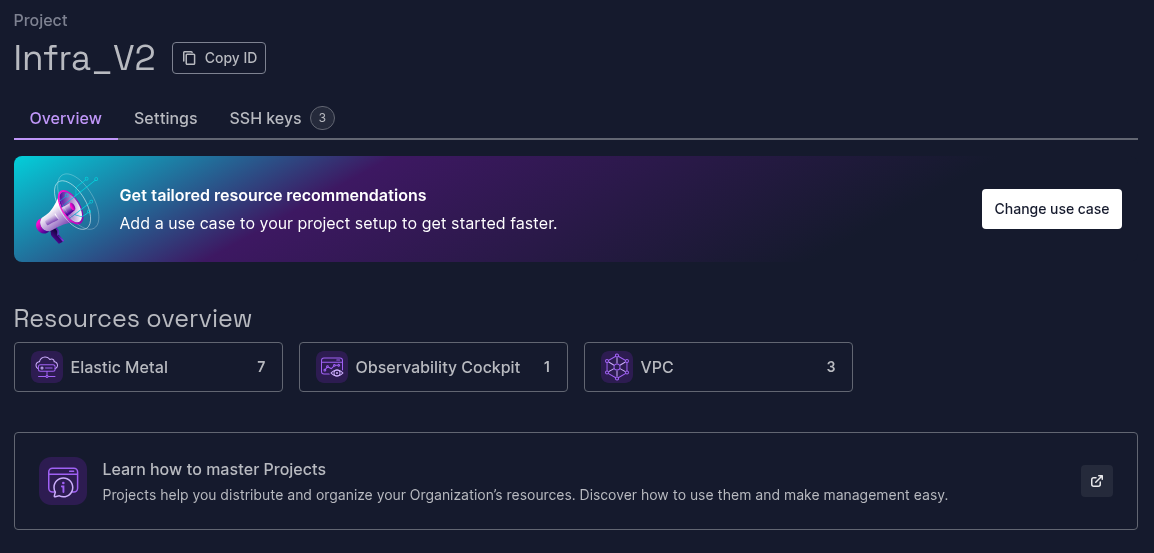
\includegraphics[width=.5\textwidth]{figures/Ressources cloud.png}
	\caption{\textit{Ressources cloud de Oneex}}
	\label{fig:Ressources cloud de Oneex}
\end{figure}
\section{Les projets informatiques de la société}
<a completer>
Oneex développe plusieurs projets informatiques stratégiques qui répondent à différents besoins métiers et techniques
\subsection{Introduction}

L’entreprise Oneex développe plusieurs projets informatiques stratégiques qui répondent à différents besoins métiers et techniques.

\subsection{Oneex Front}

Application frontend permettant la gestion des opérations, l’affichage des données et l’interaction avec les utilisateurs finaux.

\subsection{Oneex Back}

Backend exposant les API et orchestrant les processus métiers critiques.

\subsection{Oneex Scanner}

Solution logicielle dédiée à l’acquisition et à l’analyse des documents d’identité.

\subsection{Oneex ScanApp}

Application mobile ou desktop facilitant le scan et la vérification en temps réel des documents.

\subsection{Oneex CSharp}

Projet spécifique développé en C\# destiné à répondre à des besoins d’intégration ou d’outillage interne.


\chapter{Objectifs et contexte du projet}\label{chapter:objectifs_contexte}
\section{Introduction}

Dans un environnement où les systèmes d'information deviennent de plus en plus complexes et interconnectés, la maîtrise de l'infrastructure et des processus de déploiement est un enjeu majeur. Ce mémoire s'inscrit dans cette dynamique, avec pour objectif principal de concevoir et mettre en place une solution automatisée et sécurisée permettant de déployer, superviser et maintenir l'infrastructure technique de l'entreprise Oneex.

Le projet vise à répondre aux besoins opérationnels croissants, à réduire les erreurs manuelles et à garantir un haut niveau de qualité de service, tout en respectant les contraintes de sécurité et de conformité réglementaire.

\section{Cas et exemples}

Plusieurs situations rencontrées chez Oneex ont mis en évidence la nécessité d'une solution d'automatisation et de gestion centralisée de l'infrastructure. Parmi les cas récurrents :

\begin{itemize}
	\item \textbf{Problèmes de cohérence des environnements} : la configuration manuelle des serveurs engendrait des divergences entre les environnements de développement, de test et de production.
	\item \textbf{Difficultés de gestion des secrets} : le stockage et le partage des identifiants, clés d'API et certificats étaient réalisés de façon disparate, augmentant les risques de fuite.
	\item \textbf{Manque de visibilité} : l'absence d'outils de supervision unifiés complexifiait le suivi de l'état des services et la détection des incidents.
	\item \textbf{Temps de déploiement élevé} : chaque mise en place d'une infrastructure nécessitait plusieurs jours de préparation et de validation.
\end{itemize}

Ces constats ont motivé la définition d'un projet structuré et ambitieux, articulé autour de l'automatisation, de la sécurité et de l'observabilité.

\section{Les besoins fonctionnels}

Les besoins fonctionnels définissent les fonctionnalités attendues de la solution mise en œuvre. Ils se déclinent comme suit :

\begin{itemize}
	\item \textbf{Automatisation du provisioning} : création et configuration des machines virtuelles via des outils d'Infrastructure as Code (Terraform).
	\item \textbf{Gestion centralisée des configurations} : mise en place d'Ansible pour orchestrer l'installation des paquets et le paramétrage des systèmes.
	\item \textbf{Déploiement applicatif automatisé} : utilisation d'un processus GitOps avec Argo CD pour garantir la cohérence des déploiements.
	\item \textbf{Supervision et alertes} : intégration de Prometheus et Grafana pour la collecte et l'affichage des métriques.
	\item \textbf{Gestion sécurisée des secrets} : déploiement de HashiCorp Vault afin de stocker et distribuer les informations sensibles.
	\item \textbf{Mise en place d'environnements distincts} : séparation claire entre les environnements de test, de pré-production et de production.
	\item \textbf{Audits automatiques de conformité} : génération régulière de rapports d'audit afin de vérifier l'intégrité des configurations et la conformité aux standards de sécurité.
	\item \textbf{Détection précoce des erreurs} : mise en place de mécanismes permettant d'identifier rapidement les anomalies et les dysfonctionnements avant leur impact en production.
	\item \textbf{Correction automatique des erreurs et des crashs} : déploiement de processus d'auto-remédiation permettant de restaurer les services en cas d'incident.
\end{itemize}

\section{Les besoins non fonctionnels}

Les besoins non fonctionnels définissent les critères de qualité que la solution doit respecter :

\begin{itemize}
	\item \textbf{Haute disponibilité} : assurer une disponibilité supérieure à 99,9\% des services critiques.
	\item \textbf{Sécurité renforcée} : garantir la protection des données sensibles et la conformité aux standards de sécurité.
	\item \textbf{Scalabilité} : permettre l'évolution de l'infrastructure en fonction de la croissance de l'activité et de l'augmentation du nombre de clients.
	\item \textbf{Maintenabilité} : faciliter les mises à jour, les correctifs et l'évolution des configurations.
	\item \textbf{Traçabilité et auditabilité} : conserver l'historique des changements et des déploiements.
	\item \textbf{Conformité réglementaire} : respecter les normes en vigueur (RGPD, ISO 27001, etc.) et les exigences spécifiques du secteur d'activité.
	\item \textbf{Performance} : garantir des temps de réponse optimaux pour les services critiques, même en période de forte charge.
	\item \textbf{Réduction du temps de mise en production} : diminuer les délais de déploiement des nouvelles fonctionnalités.
	\item \textbf{Source unique de vérité (Single Source of Truth)} : centraliser et versionner l’ensemble des configurations, de la documentation et des états d’infrastructure dans un référentiel unique et fiable.
\end{itemize}

% \section{Le deroulement du projet}

% Le projet de mise en place d'une infrastructure automatisée s'est déroulé sur plusieurs mois, en parallèle des activités opérationnelles de l'entreprise. Il s'inscrivait dans une démarche progressive, visant à moderniser les outils et à fiabiliser les processus de déploiement et d'exploitation. Plusieurs contraintes ont dû être prises en compte, notamment la compatibilité avec l'existant, la disponibilité continue des services et la nécessité d'assurer un haut niveau de sécurité. Le planning général a été structuré en phases : conception, mise en œuvre, validation et transfert de compétences.

% \section{Objectifs du projet}

% Les objectifs principaux du projet étaient les suivants :

% \begin{itemize}
%   \item Automatiser le provisioning de l'infrastructure afin de réduire les délais de déploiement.
%   \item Centraliser et sécuriser la gestion des configurations et des secrets.
%   \item Améliorer la supervision et l'observabilité des services.
%   \item Mettre en place une approche GitOps pour les déploiements applicatifs.
%   \item Renforcer la sécurité des accès et des flux réseau.
%   \item Disposer d'environnements distincts (test, staging, production) alignés sur les bonnes pratiques DevOps.
% \end{itemize}

% Ces objectifs contribuent à la fiabilisation des opérations et à la création d'une base technique évolutive et maintenable.

\section{Architecture du projet}

L'architecture globale repose sur une infrastructure virtualisée sous Proxmox, pilotée par Terraform et configurée par Ansible. Kubernetes assure l'orchestration des conteneurs, tandis que des solutions complémentaires (Vault, Grafana, Prometheus, Loki, Tempo, Longhorn, Argo CD) viennent couvrir les besoins en sécurité, stockage et supervision.

	% Si souhaité, tu peux ajouter un schéma ici :
	%\begin{figure}[H]
	%    \centering
	%    \includegraphics[width=0.9\textwidth]{figures/architecture.png}
	%    \caption{Schéma d'architecture globale}
	%\end{figure}

	{Infrastructure as Code avec Terraform}

Terraform a été utilisé pour décrire et provisionner toute l'infrastructure. Les ressources suivantes ont été créées de façon automatisée :

\begin{itemize}
	\item Les machines virtuelles sous Proxmox (masters et workers Kubernetes, serveurs utilitaires).
	\item Les réseaux virtuels et les volumes de stockage.
	\item Les configurations initiales des systèmes (cloud-init).
\end{itemize}

Les modules Terraform ont été organisés de manière modulaire afin de pouvoir réutiliser et adapter la configuration facilement.

	{Configuration automatique avec Ansible}

Ansible a permis de configurer les serveurs après leur création. Des rôles dédiés ont été développés pour :

\begin{itemize}
	\item Installer Kubernetes (RKE2) sur les nœuds.
	\item Déployer les outils de monitoring.
	\item Configurer Vault et Consul.
	\item Appliquer les règles de sécurité et les configurations système.
\end{itemize}

Cette approche garantit une configuration homogène et reproductible.

	{GitOps avec Argo CD}

Argo CD a été mis en place pour gérer les déploiements applicatifs de manière GitOps. Chaque modification des manifestes Kubernetes dans le dépôt Git est automatiquement synchronisée avec le cluster. Cette pratique permet de disposer d’un historique complet des changements et de simplifier les rollbacks en cas de problème.

{Monitoring et observabilité avec Grafana, Prometheus, Loki et Tempo}

Le monitoring s’appuie sur Prometheus pour la collecte des métriques et Grafana pour la visualisation. Loki centralise les logs applicatifs et systèmes, tandis que Tempo gère les traces distribuées. L’ensemble forme une stack cohérente permettant d’assurer la supervision et le diagnostic des incidents.

	{Stockage distribué avec Longhorn}

Longhorn a été déployé comme solution de stockage distribué pour Kubernetes. Il fournit un stockage persistant, tolérant aux pannes, avec des fonctionnalités de snapshot et de restauration.

	{Gestion des secrets avec Vault}

Vault est utilisé comme coffre-fort centralisé pour la gestion des secrets. Il permet de stocker et de distribuer les mots de passe, tokens et certificats de manière sécurisée. Des politiques de contrôle d’accès ont été configurées pour limiter l’exposition des informations sensibles.

	{Mise en place de services internes}

Plusieurs services internes ont été installés pour répondre aux besoins quotidiens des équipes :

\begin{itemize}
	\item GitLab pour la gestion des dépôts et de l’intégration continue.
	\item Harbor comme registre privé de conteneurs.
	\item YouTrack pour le suivi des tâches et incidents.
	\item Nextcloud pour le partage sécurisé de fichiers.
\end{itemize}

Ces outils sont hébergés dans l’infrastructure Kubernetes.

	{Sécurité et gestion de pare-feu avec pfSense}

La sécurité périmétrique repose sur un pare-feu pfSense. Des règles de filtrage ont été définies pour contrôler les flux entrants et sortants, ainsi qu’un VPN pour les accès administratifs. Des mesures de surveillance des connexions ont également été mises en place.

	{Mise en place des services de test et de staging}

Des environnements spécifiques ont été créés pour permettre la validation des développements avant leur mise en production. Ces environnements reprennent l’architecture de production, facilitant les tests de montée en charge et les scénarios de validation.

	{Mise en place de la CI/CD avec GitLab CI}

GitLab CI a été configuré pour automatiser les étapes de build, test et déploiement des applications. Des pipelines ont été créés pour assurer la qualité du code et le déploiement vers les environnements Kubernetes.

	{Mise en place des services de production pour les clients}

Enfin, les environnements de production ont été finalisés et validés en respectant les exigences de performance et de sécurité. La mise en service a inclus la configuration des sauvegardes, la documentation des procédures et la formation des utilisateurs.
\section{Etude de cas et exemples}
\subsection{Cas d’Usage Concrets}

\paragraph{Exemple 1 -- Création d’un environnement complet}

\textbf{Approche classique :}
\begin{itemize}
	\item Création manuelle de trois machines virtuelles via Proxmox.
	\item Configuration réseau effectuée à la main.
	\item Copie et injection d’une clé SSH via \texttt{ssh-copy-id}.
	\item Lancement manuel d’un script d’installation.
	\item En cas d’erreur, reprise complète du processus.
\end{itemize}

\textbf{Approche Infra\_v2 :}
\begin{itemize}
	\item \texttt{terraform apply} crée automatiquement les machines virtuelles.
	\item Les clés et variables sensibles sont récupérées via Vault.
	\item Ansible configure l’ensemble : utilisateurs, sécurité, Kubernetes.
	\item Le déploiement est garanti identique à chaque exécution.
\end{itemize}

\paragraph{Exemple 2 -- Ajout d’une nouvelle application}

\textbf{Approche classique :}
\begin{itemize}
	\item Récupération du code sur une machine virtuelle.
	\item Installation manuelle des dépendances.
	\item Configuration du reverse proxy en éditant un fichier Nginx.
	\item Gestion manuelle des secrets.
	\item Vérification manuelle du démarrage du service.
\end{itemize}

\textbf{Approche Infra\_v2 :}
\begin{itemize}
	\item Définition d’un manifest Kubernetes ou d’un chart Helm.
	\item Commit dans le dépôt Git.
	\item ArgoCD détecte automatiquement le changement et effectue le déploiement.
	\item Les secrets sont injectés depuis Vault.
	\item La configuration est traçable, versionnée et cohérente.
\end{itemize}

\paragraph{Exemple 3 -- Visualisation et inspection}

\textbf{Approche classique :}
\begin{itemize}
	\item Connexion SSH sur la machine virtuelle.
	\item Parcours des fichiers de configuration.
	\item Recherche des journaux système.
	\item Vérification manuelle de l’état des services et de leur historique.
\end{itemize}

\textbf{Approche Infra\_v2 :}
\begin{itemize}
	\item Consultation du dépôt Git du projet.
	\item Inspection des manifests versionnés Kubernetes.
	\item Vérification de l’historique des commits.
	\item Observation en temps réel de la synchronisation via ArgoCD.
\end{itemize}

\paragraph{Exemple 4 -- Panne d’une machine virtuelle critique}

\textbf{Approche classique :}
\begin{itemize}
	\item En cas de saturation de la mémoire ou du disque, le service devient indisponible.
	\item Exemple réel : saturation disque sur la machine GitLab ayant bloqué l’équipe.
	\item Conséquences : interruption de la productivité, impact sur l’image, perte de confiance.
\end{itemize}

\textbf{Approche Infra\_v2 :}
\begin{itemize}
	\item Les workloads sont conteneurisés et distribués sur plusieurs nœuds Kubernetes.
	\item Si un nœud échoue, Kubernetes redémarre automatiquement les pods sur d’autres nœuds.
	\item La disponibilité est maintenue sans intervention urgente.
\end{itemize}

\paragraph{Exemple 5 -- Gestion de stacks hétérogènes}

\textbf{Approche classique :}
\begin{itemize}
	\item Multiplicité des environnements techniques :
	      \begin{itemize}
		      \item Docker
		      \item Python et \texttt{pip}
		      \item Services installés via \texttt{apt}
	      \end{itemize}
	\item La connaissance des procédures est dispersée entre différents intervenants.
\end{itemize}

\textbf{Approche Infra\_v2 :}
\begin{itemize}
	\item Chaque application dispose d’un manifest Kubernetes ou d’un chart Helm.
	\item Les dépendances sont déclarées et isolées dans des conteneurs.
	\item Le déploiement est homogène et automatisé via GitOps.
	\item Plus besoin de maîtriser des commandes spécifiques à chaque stack.
\end{itemize}

\paragraph{Exemple 6 -- Retour en arrière après une erreur}

\textbf{Approche classique :}
\begin{itemize}
	\item Identification manuelle de l’erreur.
	\item Correction parfois empirique.
	\item Restauration longue (rollback manuel, restauration de snapshot).
\end{itemize}

\textbf{Approche Infra\_v2 :}
\begin{itemize}
	\item \texttt{git revert} permet de revenir à un état stable.
	\item ArgoCD synchronise automatiquement l’environnement.
	\item Le retour arrière est rapide et traçable.
\end{itemize}

\paragraph{Exemple 7 -- Mise à jour sans interruption de service}

\textbf{Approche classique :}
\begin{itemize}
	\item Mise à jour en place avec risque d’indisponibilité.
	\item Obligation de programmer une plage de maintenance.
\end{itemize}

\textbf{Approche Infra\_v2 :}
\begin{itemize}
	\item Kubernetes réalise des \emph{rolling updates}.
	\item Les pods sont remplacés progressivement.
	\item Pas d’interruption visible pour les utilisateurs.
	\item Rollback automatique en cas de problème.
\end{itemize}

\subsection*{Résumé des bénéfices}

Ces exemples démontrent l’intérêt de l’approche \textbf{Infra\_v2}, qui apporte des avantages significatifs :

\begin{itemize}
	\item Automatisation et reproductibilité totales.
	\item Sécurité centralisée des secrets.
	\item Déploiement et rollback versionnés, contrôlés et traçables.
	\item Résilience et haute disponibilité natives.
	\item Réduction drastique des erreurs humaines.
	\item Visibilité accrue sur l’état des applications et de l’infrastructure.
	\item Scalabilité et maintenance simplifiées.
\end{itemize}

\section{Conclusion}
Ce projet de mise en place d'une infrastructure automatisée et sécurisée pour Oneex a permis de répondre aux enjeux opérationnels et stratégiques de l'entreprise. En intégrant des outils modernes et des pratiques DevOps, il a été possible d'améliorer la fiabilité, la sécurité et la rapidité des déploiements.
L'architecture mise en place offre une base solide pour l'évolution future des services, tout en
assurant une gestion centralisée et sécurisée des configurations et des secrets. Les équipes disposent désormais d'un environnement cohérent, scalable et maintenable, capable de s'adapter aux besoins croissants de l'entreprise.
Ce mémoire présente les différentes étapes de conception et de mise en œuvre de cette solution, ainsi que
les résultats obtenus. Il met en lumière l'importance de l'automatisation, de la sécurité et de l'observabilité dans la gestion des infrastructures modernes, et ouvre la voie à de futures améliorations et innovations au sein de Oneex.
Ce projet s'inscrit dans une démarche continue d'amélioration et d'optimisation des processus
et expliquer la securité par design vs la securité par obscurité. Il est essentiel de continuer à investir dans la formation des équipes, l'évolution des outils et la mise en place de bonnes pratiques pour garantir la pérennité et la sécurité de l'infrastructure.
\subsection{Perspectives d'évolution}

L’approche \textbf{Infra\_v2} ouvre la voie à plusieurs évolutions futures permettant d’améliorer encore la performance, la fiabilité et la maintenabilité des systèmes :

\begin{itemize}
	\item \textbf{Renforcement de l’automatisation} : intégrer davantage de processus automatisés (tests d’intégration, vérifications de sécurité, audits de conformité) dans les pipelines CI/CD.

	\item \textbf{Observabilité avancée} : enrichir la télémétrie avec OpenTelemetry afin de collecter traces, métriques et logs de manière unifiée, facilitant le diagnostic en temps réel.

	\item \textbf{Scalabilité horizontale} : étendre la capacité de la plateforme Kubernetes en ajoutant dynamiquement des nœuds selon la charge.

	\item \textbf{Sécurité renforcée} : généraliser le chiffrement des communications internes, la rotation automatique des secrets et le principe de moindre privilège.

	\item \textbf{Standardisation des workflows} : promouvoir l’utilisation systématique de GitOps pour toutes les équipes afin de garantir une cohérence des pratiques de déploiement.

	\item \textbf{Optimisation des coûts} : introduire des mécanismes de scaling automatique et de surveillance des ressources afin de réduire les coûts d’infrastructure.
\end{itemize}

Ces perspectives s’inscrivent dans une démarche d’amélioration continue visant à industrialiser et fiabiliser la gestion des environnements techniques.

\subsection{Les points forts et faibles du point de vue technique et organisationnel}

\textbf{Points forts techniques :}
\begin{itemize}
	\item Infrastructure déclarative et versionnée, facilitant la reproductibilité et la traçabilité des changements.
	\item Automatisation complète du cycle de vie des environnements (provisionnement, configuration, déploiement).
	\item Haute disponibilité native grâce à Kubernetes et au découplage des composants.
	\item Facilité de rollback rapide en cas d’erreur.
	\item Intégration transparente de la gestion des secrets via Vault.
\end{itemize}

\textbf{Points faibles techniques :}
\begin{itemize}
	\item Courbe d’apprentissage élevée pour maîtriser l’ensemble des outils (Terraform, Ansible, Kubernetes, ArgoCD).
	\item Complexité accrue du système global nécessitant une veille technologique régulière.
	\item Dépendance à l’intégrité des outils d’orchestration (un dysfonctionnement de GitOps ou de l’API Kubernetes peut impacter la disponibilité).
\end{itemize}

\textbf{Points forts organisationnels :}
\begin{itemize}
	\item Processus standardisés réduisant les erreurs humaines.
	\item Visibilité complète des configurations via Git.
	\item Meilleure collaboration entre les équipes grâce à une approche déclarative et transparente.
	\item Accélération des cycles de déploiement.
\end{itemize}

\textbf{Points faibles organisationnels :}
\begin{itemize}
	\item Nécessité d’une conduite du changement importante pour faire adopter les nouveaux outils.
	\item Risque de silos de compétences si la montée en compétence n’est pas homogène au sein des équipes.
	\item Temps initial d’implémentation élevé pour mettre en place les pipelines et standardiser les pratiques.
\end{itemize}


\chapter{Conception et automatisation de l’infrastructure}\label{chapter:iac}
\section{Introduction}

La conception et la mise en œuvre d’une infrastructure moderne reposent aujourd’hui sur l’automatisation complète des processus de création, de configuration et de sécurisation des environnements. Cette approche permet de garantir la cohérence, la traçabilité et la reproductibilité des déploiements tout en réduisant la complexité opérationnelle.

Ce chapitre présente la démarche adoptée pour concevoir et automatiser l’infrastructure du projet, en s’appuyant sur les principes de l’Infrastructure as Code et sur des outils spécialisés. Il expose dans un premier temps les technologies sélectionnées, telles que Proxmox, Terraform, Cloud-init, Ansible, Vault et Consul, qui constituent les fondations techniques de l’architecture. La suite du chapitre décrit la mise en œuvre progressive des différents composants : la gestion des secrets, la création automatisée des machines virtuelles, la préparation des inventaires et la configuration des services.

Par ailleurs, l’usage de Vault comme solution centralisée de gestion des secrets répond à la nécessité de renforcer la sécurité et la traçabilité des informations sensibles au sein de l’infrastructure. Contrairement aux mécanismes de stockage natifs (par exemple les secrets Kubernetes ou les variables d’environnement chiffrées de manière basique), Vault permet de chiffrer systématiquement les données au repos et en transit, de générer des identifiants dynamiques à durée de vie limitée et de contrôler finement les accès via des politiques granulaires. Cette approche réduit les risques de compromission, simplifie la rotation périodique des secrets et garantit que ceux-ci ne transitent jamais en clair dans les dépôts de code ou les configurations partagées. L’intégration de Vault s’inscrit donc pleinement dans la logique Infrastructure as Code et contribue à élever le niveau de sécurité tout en automatisant la distribution des secrets.

Enfin, une attention particulière est portée aux aspects réseau et à la sécurisation des flux, avec l’intégration de pare-feu, de mécanismes d’équilibrage de charge et de politiques de segmentation. Cette démarche globale vise à démontrer qu’il est possible de déployer une infrastructure complète et sécurisée de manière déclarative, tout en facilitant son évolutivité et sa maintenance.
\section{Les outils utilisés pour l’infrastructure as code}

\subsection{Proxmox}

Proxmox Virtual Environment (Proxmox VE) est une plateforme open source de virtualisation et de gestion d’infrastructure qui combine la virtualisation basée sur des machines virtuelles (KVM) et la conteneurisation légère (LXC) dans une interface unifiée. Elle offre une solution complète pour déployer et administrer des environnements virtualisés, qu’ils soient utilisés en laboratoire, en PME ou dans des centres de données. Proxmox se distingue par sa simplicité de mise en œuvre, sa richesse fonctionnelle et sa capacité à fédérer plusieurs nœuds dans un cluster haute disponibilité.

Proxmox répond à plusieurs enjeux stratégiques : rationalisation des ressources matérielles par la mutualisation, réduction des coûts grâce à une solution libre, amélioration de la flexibilité opérationnelle et simplification de la gestion des infrastructures. Son interface web ergonomique permet de piloter l’ensemble des ressources, de planifier les sauvegardes et de superviser les performances.

D’un point de vue technique, Proxmox repose sur plusieurs composantes clés :
\begin{itemize}
	\item \textbf{KVM (Kernel-based Virtual Machine)} : moteur de virtualisation complète.
	\item \textbf{LXC (Linux Containers)} : conteneurisation système légère.
	\item \textbf{Ceph Storage} : stockage distribué intégré et hautement disponible.
	\item \textbf{Cluster Management} : fédération et basculement automatique.
	\item \textbf{Interface Web et API REST} : administration centralisée.
	\item \textbf{Sauvegardes et snapshots} : gestion de la résilience.
\end{itemize}

\textbf{Cas d’utilisation} : déploiement d’un cluster de trois nœuds Proxmox avec stockage Ceph pour héberger des machines virtuelles critiques en haute disponibilité.

\subsection{Terraform}

Terraform est un outil open source d’Infrastructure as Code développé par HashiCorp. Il permet de définir et de provisionner des ressources complètes sous forme de code déclaratif, avec un modèle unifié pour divers fournisseurs (clouds publics, hyperviseurs privés).

Terraform répond à plusieurs enjeux : accélération du provisioning, fiabilisation des configurations et maîtrise des environnements. Il repose sur des concepts clés :
\begin{itemize}
	\item \textbf{Fichiers de configuration (HCL)} : description de l’état souhaité.
	\item \textbf{Providers} : modules d’interface avec les APIs.
	\item \textbf{State file} : enregistrement des ressources créées.
	\item \textbf{Plan d’exécution} et \textbf{apply} : gestion des changements.
	\item \textbf{Modules et workspaces} : factorisation et isolation.
\end{itemize}

\textbf{Cas d’utilisation} : provisionner un cluster Kubernetes sur Proxmox avec un réseau et des volumes configurés.

% \subsection{Cloud-init}

% Cloud-init est un outil d’initialisation automatique des machines virtuelles lors du premier démarrage. Il est supporté par la plupart des plateformes cloud et hyperviseurs, et permet :
% \begin{itemize}
% 	\item La configuration réseau.
% 	\item La création d’utilisateurs et de clés SSH.
% 	\item L’installation de paquets et le lancement de scripts.
% \end{itemize}

% Cloud-init contribue à standardiser les environnements et réduire les délais de mise en service.

% \textbf{Cas d’utilisation} : automatiser l’installation de Docker et la configuration réseau d’une instance Proxmox.

\subsection{Ansible}

Ansible est un outil open source d’automatisation et de configuration des systèmes, basé sur un langage déclaratif YAML et une architecture agentless (connexion SSH). Il permet de :
\begin{itemize}
	\item Définir des playbooks réutilisables.
	\item Orchestrer la configuration de plusieurs hôtes.
	\item Gérer des inventaires et des variables.
	\item Assurer la traçabilité des opérations.
\end{itemize}

\textbf{Cas d’utilisation} : configurer des serveurs applicatifs, installer les dépendances et sécuriser les accès.

\subsection{Vault}

Vault est un gestionnaire de secrets développé par HashiCorp, conçu pour sécuriser, stocker et contrôler l’accès aux informations sensibles telles que les identifiants, les clés d’API ou les certificats. Il centralise le cycle de vie des secrets au sein d’un système unique et auditable, tout en offrant des capacités de distribution dynamique et de rotation automatique.

\textbf{Principales fonctionnalités} :
\begin{itemize}
	\item Chiffrement systématique des données au repos et en transit.
	\item Génération dynamique de credentials à durée de vie limitée.
	\item Contrôle d’accès fin grâce à des politiques (ACL) granulaires.
	\item Rotation périodique et automatique des secrets.
	\item Audit complet des opérations et des accès.
\end{itemize}

\paragraph{Concepts de base}

Vault repose sur plusieurs concepts fondamentaux :

\begin{itemize}
	\item \textbf{Seal et Unseal} : lors de son démarrage, Vault est scellé (sealed). Dans cet état, aucune donnée ne peut être lue ou écrite. Le processus d’unseal consiste à déverrouiller Vault en fournissant une combinaison de clés de déchiffrement (unseal keys) générées lors de l’initialisation. Ce mécanisme s’appuie sur l’algorithme de \emph{Shamir’s Secret Sharing}, qui divise la clé maîtresse en fragments distribués à différents opérateurs. Cela garantit qu’aucun individu ne détient seul la capacité de déverrouiller le système. La nécessité d’unseal manuellement après un redémarrage contribue à limiter l’exposition en cas de compromission physique ou de coupure d’alimentation.
	\item \textbf{Backends de stockage} : Vault peut s’appuyer sur différents backends de stockage (par exemple Consul, fichiers locaux, Amazon S3) pour persister ses données chiffrées. Le choix du backend influence les performances, la disponibilité et la tolérance aux pannes.
	\item \textbf{Secrets Engines} : ce sont les composants responsables de la gestion des secrets. Certains engines fournissent du stockage statique (par exemple les clés stockées manuellement), d’autres génèrent des secrets dynamiques à la demande (par exemple des credentials temporaires pour une base de données).
	\item \textbf{Auth Methods} : ces méthodes définissent comment les utilisateurs ou applications s’authentifient auprès de Vault. Il peut s’agir de tokens statiques, d’authentification AppRole, de certificats TLS ou d’intégrations avec Kubernetes.
	\item \textbf{Policies} : les politiques d’accès contrôlent avec précision ce que chaque entité est autorisée à faire. Elles définissent les droits de lecture, d’écriture ou de suppression sur des chemins spécifiques.
\end{itemize}

\paragraph{Design de sécurité}

Vault adopte une approche de sécurité par défaut :
\begin{itemize}
	\item Toutes les données sont chiffrées avec une clé maîtresse qui n’est jamais stockée en clair.
	\item Chaque requête est soumise à une évaluation des politiques d’accès.
	\item Les secrets peuvent être versionnés et révoqués à tout moment.
	\item Les logs d’audit permettent de tracer finement chaque opération.
\end{itemize}
Ce modèle de sécurité réduit le risque d’exposition accidentelle et renforce la conformité aux exigences réglementaires.

\paragraph{Exemple d’utilisation}

Vault est particulièrement adapté pour :
\begin{itemize}
	\item Stocker et distribuer les tokens Kubernetes nécessaires à l’accès au cluster.
	\item Générer des credentials temporaires pour une base de données PostgreSQL.
	\item Chiffrer les certificats TLS utilisés par des applications.
	\item Mettre en place un PKI interne pour l’émission automatique de certificats.
\end{itemize}

\paragraph{Bonnes pratiques de sécurité}

Pour garantir un niveau de protection élevé, il est recommandé de :
\begin{itemize}
	\item Distribuer les clés de scellage (unseal keys) à plusieurs opérateurs de confiance afin de prévenir tout point de défaillance individuel.
	\item Configurer une rotation périodique des clés maîtresses.
	\item Limiter strictement l’accès aux méthodes d’authentification les plus sensibles.
	\item Activer et surveiller systématiquement les logs d’audit.
	\item S’assurer que le backend de stockage est hautement disponible et correctement sécurisé.
\end{itemize}

\paragraph{Limitations et vigilance}

Si Vault n’est pas configuré de manière rigoureuse, il peut devenir un point unique de défaillance et un vecteur d’attaque majeur. La compromission d’un nœud ou la perte des clés de déchiffrement peut entraîner une indisponibilité prolongée, voire la perte irrémédiable de certains secrets. Il est donc essentiel d’envisager des scénarios de récupération, tels que la sauvegarde chiffrée des données et la documentation des procédures d’unseal.
% \subsection{Consul}

% Consul est une solution de service discovery, de configuration distribuée et de service mesh développée par HashiCorp. Elle permet de centraliser la gestion dynamique des services et de renforcer la cohérence des environnements déployés. Consul apporte plusieurs fonctionnalités complémentaires à Vault et s’intègre naturellement dans les architectures automatisées.

% \paragraph{Principales fonctionnalités}

% Les principales capacités de Consul sont les suivantes :
% \begin{itemize}
% 	\item \textbf{Découverte automatique des services} : Consul maintient un catalogue des services enregistrés, avec leurs adresses et ports associés, facilitant leur détection et leur utilisation par d’autres composants.
% 	\item \textbf{Supervision de l’état des services} : le système exécute des contrôles de santé (health checks) qui permettent de vérifier en continu la disponibilité et le bon fonctionnement des instances.
% 	\item \textbf{Stockage clé-valeur} : Consul fournit un KV store distribué, utilisé pour stocker des paramètres de configuration ou des informations dynamiques accessibles par les applications.
% 	\item \textbf{Service mesh sécurisé} : grâce à l’intégration avec Envoy, Consul offre un plan de contrôle permettant de chiffrer le trafic inter-services, d’implémenter des politiques d’accès et de réaliser du routage avancé.
% \end{itemize}

\paragraph{Architecture et composants}

Consul repose sur une architecture distribuée, composée de plusieurs éléments :
\begin{itemize}
	\item \textbf{Agents} : chaque nœud du cluster exécute un agent Consul, qui peut être configuré en mode client ou serveur.
	\item \textbf{Serveurs} : les serveurs Consul assurent la cohérence des données à l’aide d’un consensus basé sur le protocole Raft.
	\item \textbf{Catalogue de services} : une base de données en temps réel contenant les informations sur tous les services enregistrés et leur état de santé.
	\item \textbf{KV Store} : un espace de stockage distribué, utilisé pour partager des données de configuration.
	\item \textbf{Connect} : le composant de service mesh qui gère l’émission de certificats TLS, le chiffrement du trafic et le contrôle des autorisations.
\end{itemize}

\paragraph{Mécanismes et cas d’usage}

Consul propose plusieurs mécanismes qui répondent à des besoins spécifiques :

\begin{itemize}
	\item \emph{Service discovery} : lorsqu’un service s’enregistre auprès de Consul, il devient automatiquement visible pour les clients qui peuvent interroger l’API DNS ou HTTP afin de récupérer ses coordonnées.
	\item \emph{Health checks} : chaque enregistrement de service peut être associé à un ou plusieurs tests de disponibilité. Si un service échoue aux contrôles, il est retiré du catalogue actif.
	\item \emph{KV Store} : les applications peuvent récupérer dynamiquement des paramètres ou configurations partagées (par exemple des variables d’environnement ou des endpoints).
	\item \emph{Consul Template} : cet outil surveille le KV store et les catalogues, puis génère automatiquement des fichiers de configuration lorsque des changements surviennent.
	\item \emph{Service mesh} : Consul Connect émet des certificats mTLS, configure les proxys Envoy et applique des politiques d’accès qui définissent quels services sont autorisés à communiquer.
\end{itemize}

\textbf{Exemple d’utilisation} : synchroniser dynamiquement les configurations applicatives avec Consul Template, mettre à jour les fichiers de configuration NGINX lorsque de nouveaux services sont enregistrés, ou établir un canal de communication chiffré entre des microservices.

\paragraph{Bonnes pratiques de sécurité}

Pour tirer parti des fonctionnalités de Consul tout en maintenant un niveau élevé de sécurité, il est recommandé de :
\begin{itemize}
	\item Activer le chiffrement TLS pour toutes les communications inter-nœuds.
	\item Protéger l’interface HTTP API par une ACL stricte.
	\item Mettre en place des politiques de token management et de rotation régulière des secrets.
	\item Limiter l’accès aux agents et serveurs Consul au sein d’un réseau privé.
	\item Activer l’audit des requêtes et opérations critiques.
\end{itemize}

\paragraph{Limitations et vigilance}

De meme que vault , malgré sa richesse fonctionnelle, Consul peut devenir un point unique de coordination : une indisponibilité du cluster impacte la découverte des services et la cohérence des configurations. De plus, une configuration incorrecte des ACL ou des intentions (politiques de service mesh) peut entraîner des fuites d’informations ou des interruptions de service. Il est donc essentiel de soigner le dimensionnement du cluster, de planifier des sauvegardes régulières et de tester les scénarios de bascule.

\section{Mise en place des concepts de l'infrastructure en code}

La mise en œuvre d'une infrastructure déclarative repose sur une combinaison d'outils spécialisés qui permettent d'automatiser l'ensemble du cycle de vie des environnements techniques. Cette approche favorise la cohérence, la traçabilité et la reproductibilité des déploiements.
Les sections suivantes décrivent les principales étapes mises en place dans le projet.

\subsection{Préparation des secrets avec Vault}

Dans une architecture moderne, la gestion sécurisée des informations sensibles (mots de passe, clés d'API, certificats) est un enjeu majeur.
Pour répondre à cette problématique, l'outil HashiCorp Vault a été utilisé comme coffre-fort centralisé.

Vault a été configuré en mode \textit{server} avec un stockage interne et une politique de chiffrement des données au repos. Les secrets sont créés et organisés dans des chemins logiques (\texttt{secret/}, \texttt{kv/}) permettant de les isoler par projet ou par environnement (développement, production).

L'accès à Vault est contrôlé par des policies granulaires, et l'authentification des outils d'automatisation (Terraform, Ansible) s'effectue via des tokens dynamiques ou l'approche AppRole.
Cette centralisation simplifie la rotation des secrets et réduit les risques liés aux configurations manuelles.

\subsection{Création de templates de machines virtuelles}

Afin de garantir l'uniformité des systèmes de base, des templates de machines virtuelles ont été préparés sur Proxmox.
Ces templates incluent :
\begin{itemize}
	\item Le système d'exploitation minimal (par exemple Debian ou Ubuntu LTS).
	\item Les mises à jour de sécurité appliquées.
	\item Les dépendances de base (cloud-init, agents QEMU, agents SPICE et agents ).
	\item La configuration des clés SSH nécessaires à l'automatisation.
\end{itemize}

L'utilisation de ces modèles préconfigurés permet de créer rapidement de nouvelles instances sans avoir à répéter les étapes de préparation initiale.
Cette approche contribue à standardiser le socle technique et à réduire le temps de provisionnement.

\subsection{Création des machines virtuelles à travers Terraform}

La création automatisée des machines virtuelles est orchestrée par Terraform.
Les ressources sont décrites sous forme de fichiers HCL (\textit{HashiCorp Configuration Language}) qui précisent :
\begin{itemize}
	\item La taille et le nombre de vCPU et de mémoire.
	\item Le réseau et les interfaces associées.
	\item Le disque principal et son format.
	\item Le template de base à cloner.
\end{itemize}

L'exécution de \texttt{terraform apply} permet de matérialiser l'infrastructure déclarée.
Cette étape est également responsable de l'injection initiale des métadonnées (par exemple, le nom de l'instance, l'identifiant d'environnement).
Grâce à Terraform, la création des VMs est reproductible et contrôlée dans le temps.

\subsection{Préparation automatique des inventaires}

Après le provisionnement des ressources, la préparation des inventaires est essentielle pour permettre à Ansible de prendre le relais.
Pour ce faire, un script d'automatisation collecte dynamiquement les informations des machines créées (adresses IP, identifiants, groupes logiques) et génère un inventaire au format YAML compatible avec Ansible.

Cette génération automatisée évite les erreurs liées aux manipulations manuelles et garantit que l'inventaire reflète toujours l'état réel de l'infrastructure.
L'inventaire est versionné dans un dépôt Git, renforçant la traçabilité des évolutions.

\subsection{Configuration automatique des machines virtuelles avec Ansible}

Une fois les inventaires préparés, Ansible est utilisé pour configurer les machines virtuelles de manière déclarative.
Les rôles et playbooks appliquent notamment :
\begin{itemize}
	\item La création des utilisateurs et des groupes.
	\item La configuration du pare-feu et des règles de sécurité.
	\item L'installation des paquets requis.
	\item Le déploiement des configurations d’applications et des services système.
\end{itemize}

L'exécution d'Ansible est idempotente, garantissant que les machines convergent toujours vers l'état souhaité, quelle que soit leur configuration initiale.
Les variables sensibles sont injectées de manière sécurisée via Vault.

\section{Outils de réseau, exposition des services et sécurité}

Le bon fonctionnement d'une infrastructure passe par une gestion rigoureuse du réseau et une exposition contrôlée des services.
Dans le projet, plusieurs composants et bonnes pratiques ont été mis en œuvre :

\begin{itemize}
	\item \textbf{Réseau virtuel et segmentation} : les machines sont placées dans des VLANs distincts afin de séparer les environnements (production, développement) et de limiter les flux inter-zones.
	\item \textbf{Reverse proxy et ingress} : l’exposition des services HTTP(S) s’effectue via des ingress controllers Kubernetes ou des reverse proxies tels que NGINX. Ces composants assurent le routage, la terminaison TLS et l’équilibrage de charge.
	\item \textbf{Certificats TLS} : les certificats sont gérés automatiquement grâce à l’intégration de Let’s Encrypt ou Vault PKI, garantissant la sécurité des échanges.
	\item \textbf{Pare-feu et contrôle des accès} : des règles strictes sont appliquées sur les hôtes et les pods, combinant iptables, security groups et Network Policies Kubernetes.
	\item \textbf{Monitoring et logs} : la collecte centralisée des logs réseau et la supervision des connexions permettent d’anticiper les incidents et de renforcer la sécurité.
\end{itemize}

Cette approche cohérente assure une exposition minimale des services au public et une sécurité renforcée tout en maintenant une haute disponibilité.

\paragraph{Firewall pfSense}

Pour renforcer la sécurité réseau, plusieurs architectures avec \textbf{pfSense} (distribution libre spécialisée dans les fonctions de pare-feu et de routage) ont été considérées. Voici les options analysées :

\subparagraph{Scénario 1 : pfSense en VM ou LXC dédié sur Proxmox}

\begin{itemize}
	\item pfSense est déployé comme une VM avec deux interfaces réseau (WAN et LAN).
	\item Elle agit comme passerelle pour toutes les autres VMs.
	\item Avantage : isolation logique et grande flexibilité.
	\item Limite : dépendance à Proxmox (si le nœud tombe, le firewall aussi).
\end{itemize}

\subparagraph{Scénario 2 : pfSense sur un serveur physique séparé}

\begin{itemize}
	\item pfSense fonctionne comme appliance physique devant le cluster.
	\item Avantage : indépendance vis-à-vis de la plateforme de virtualisation.
	\item Permet de filtrer tout le trafic entrant/sortant.
	\item Limite : nécessite du matériel dédié, plus de câblage et de gestion physique.
\end{itemize}

\begin{figure}[H]
	\centering
	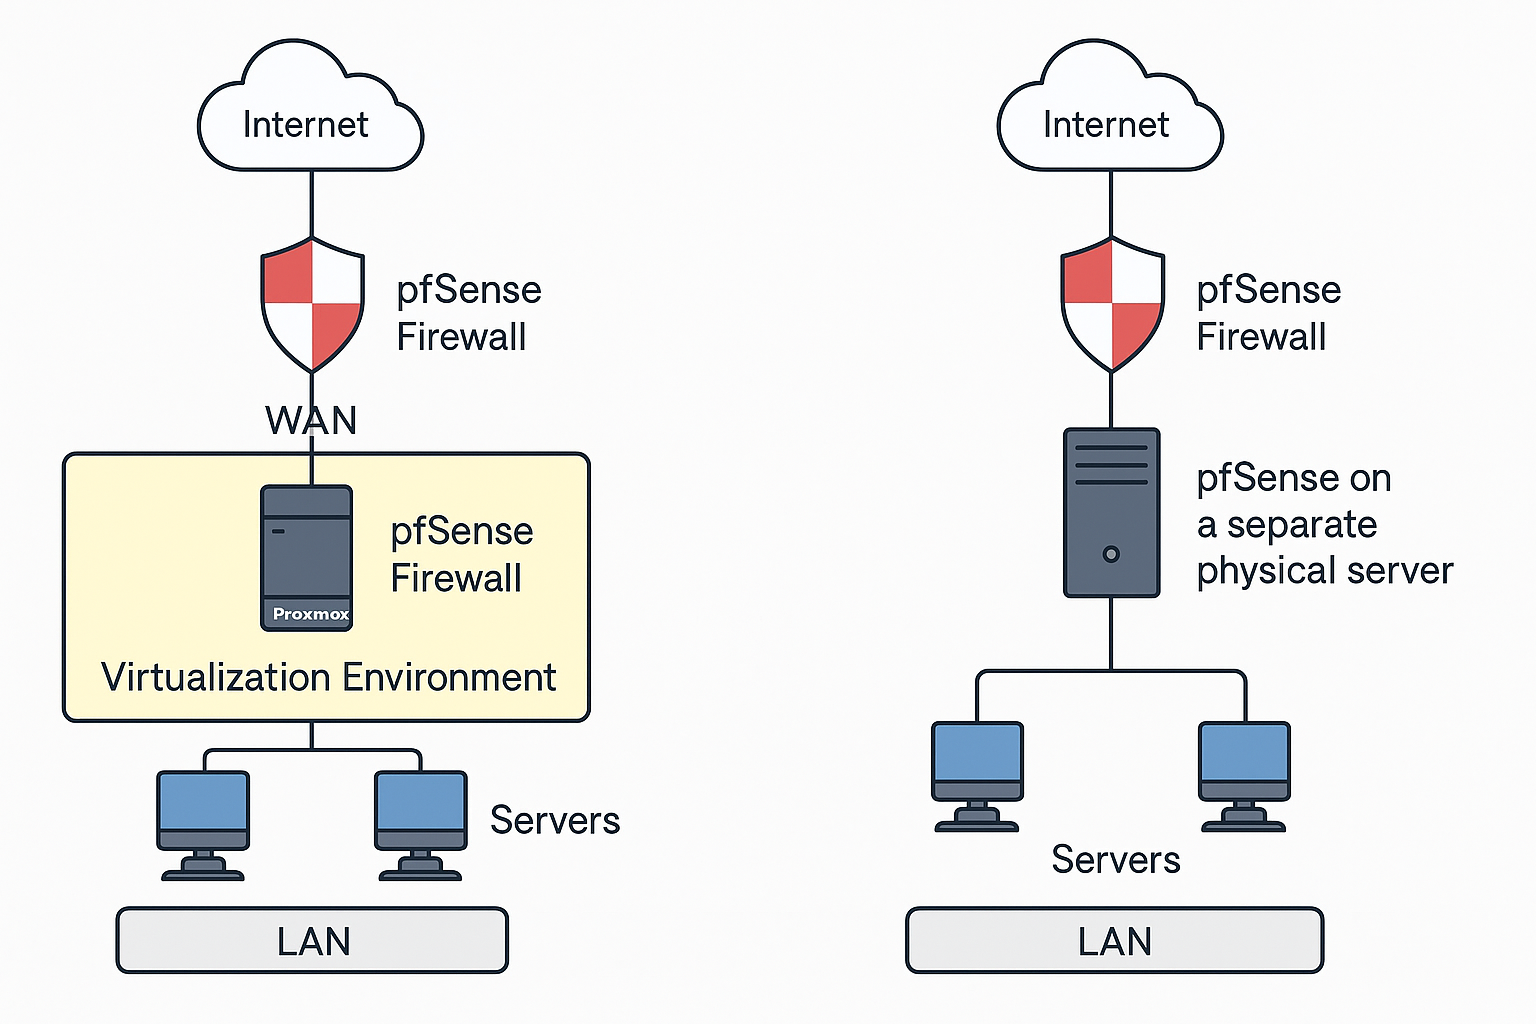
\includegraphics[width=0.85\textwidth]{figures/choix implementation pfsense.png}
	\caption{Comparaison des architectures d'intégration de pfSense}
\end{figure}

Le tableau \ref{tab:pfsense_arch} résume les avantages et inconvénients de chaque approche :

\begin{longtable}{|p{4.5cm}|p{3.5cm}|p{3cm}|p{3.5cm}|}
	\caption{\it{Comparaison des modes d’intégration de pfSense}}
	\label{tab:pfsense_arch}                                                                                                               \\ \hline
	\textbf{Architecture}        & \textbf{Isolation} & \textbf{Résilience} & \textbf{Commentaires}                                        \\ \hline
	\endfirsthead
	\multicolumn{4}{l}{\tablename\ \thetable\ -- \textit{Suite}}                                                                           \\ \hline
	\textbf{Architecture}        & \textbf{Isolation} & \textbf{Résilience} & \textbf{Commentaires}                                        \\ \hline
	\endhead
	\endfoot
	\hline
	\endlastfoot

	VM dédiée ou LXC sur Proxmox & Élevée             & Moyenne             & Facile à déployer, centralisé, mais dépend du nœud Proxmox.  \\ \hline
	Appliance physique séparée   & Très élevée        & Très élevée         & Solution professionnelle, coûteuse, idéale pour multi-sites. \\ \hline
\end{longtable}

\paragraph{Choix retenu et justification}

Dans le contexte de l’infrastructure actuelle de Oneex, c’est le \textbf{scénario 1} (déploiement de pfSense dans une VM dédiée sur Proxmox) qui a été retenu. Cette approche présente plusieurs avantages majeurs en adéquation avec l’architecture existante :

\begin{itemize}
	\item Elle permet d’\textbf{intégrer pleinement le pare-feu dans le réseau interne}, avec un contrôle précis sur le filtrage inter-VLAN et la segmentation réseau.
	\item pfSense peut \textbf{établir des connexions VPN de type IPsec} entre les différents LANs internes de l’entreprise, assurant ainsi une interconnexion sécurisée des environnements distants.
	\item Cette configuration est \textbf{hautement personnalisable} : routage, NAT, tunnels chiffrés, DHCP statique, filtrage applicatif, etc., tout en restant cohérente avec la logique IaaS de Proxmox.
\end{itemize}

Malgré une résilience moyenne (liée à sa dépendance à Proxmox), cette solution constitue un compromis optimal entre flexibilité, centralisation et sécurité, tout en réduisant les coûts matériels. Elle est également plus facile à maintenir et à intégrer dans les processus automatisés de l'infrastructure.

\subsection{Réseau de Kubernetes}

Le réseau Kubernetes est un élément fondamental qui permet la communication entre les différents composants du cluster et les applications qui y sont déployées. Il repose sur plusieurs concepts clés visant à simplifier la connectivité et à assurer l’isolation logique des workloads.

\paragraph{Modèle de réseau plat}

Kubernetes adopte un modèle de réseau dit \emph{plat}, dans lequel :
\begin{itemize}
	\item Chaque \textbf{pod} reçoit une adresse IP unique.
	\item Tous les pods peuvent communiquer entre eux, sans traduction d’adresses (NAT).
	\item Les pods peuvent accéder aux services exposés par d’autres pods, quel que soit le nœud sur lequel ils s’exécutent.
\end{itemize}
\begin{figure}[H]
	\centering
	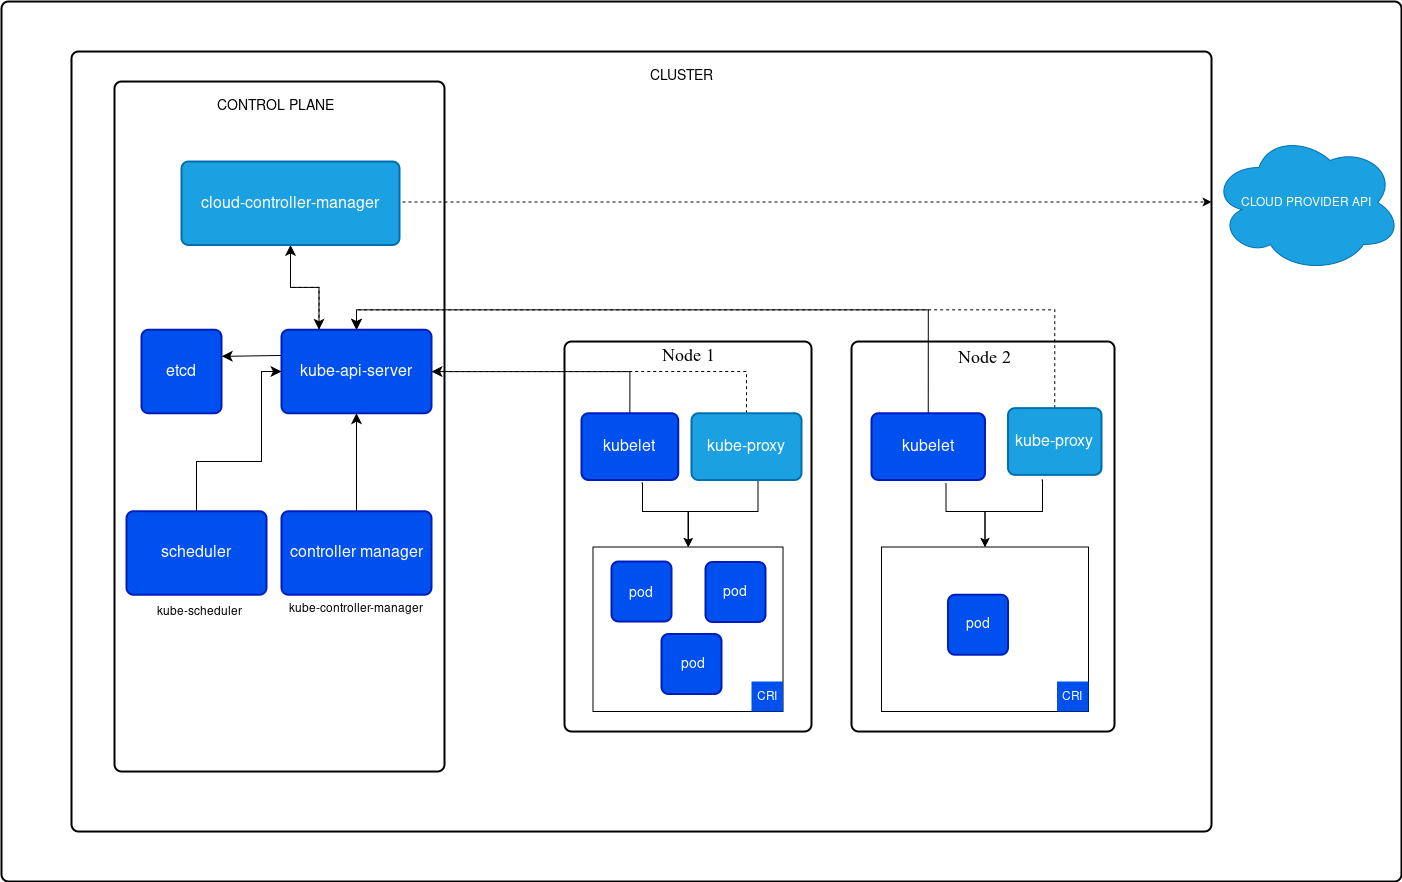
\includegraphics[width=0.85\textwidth]{figures/kubernetes-cluster-architecture.png}
	\caption{Architecture d'un cluster Kubernetes}
\end{figure}
Ce modèle vise à réduire la complexité des communications et à permettre aux applications de se comporter comme si elles fonctionnaient sur un même réseau local.

\paragraph{CNI (Container Network Interface)}

Pour mettre en œuvre le modèle réseau, Kubernetes s’appuie sur des plugins CNI (Container Network Interface).
Ces plugins sont responsables de :
\begin{itemize}
	\item L’attribution des adresses IP aux pods.
	\item La configuration des routes réseau.
	\item L’application des règles de filtrage ou d’isolation.
\end{itemize}
Parmi les solutions CNI les plus courantes, on peut citer Calico, Flannel, Cilium et Weave.

\paragraph{Services et exposition réseau dans Kubernetes}

Kubernetes introduit l’objet \texttt{Service}, utilisé pour exposer un ensemble de pods via une abstraction réseau stable (nom DNS et IP virtuelle). Cela permet de découpler la logique de service de l’adressage dynamique des pods.

\begin{figure}[H]
	\centering
	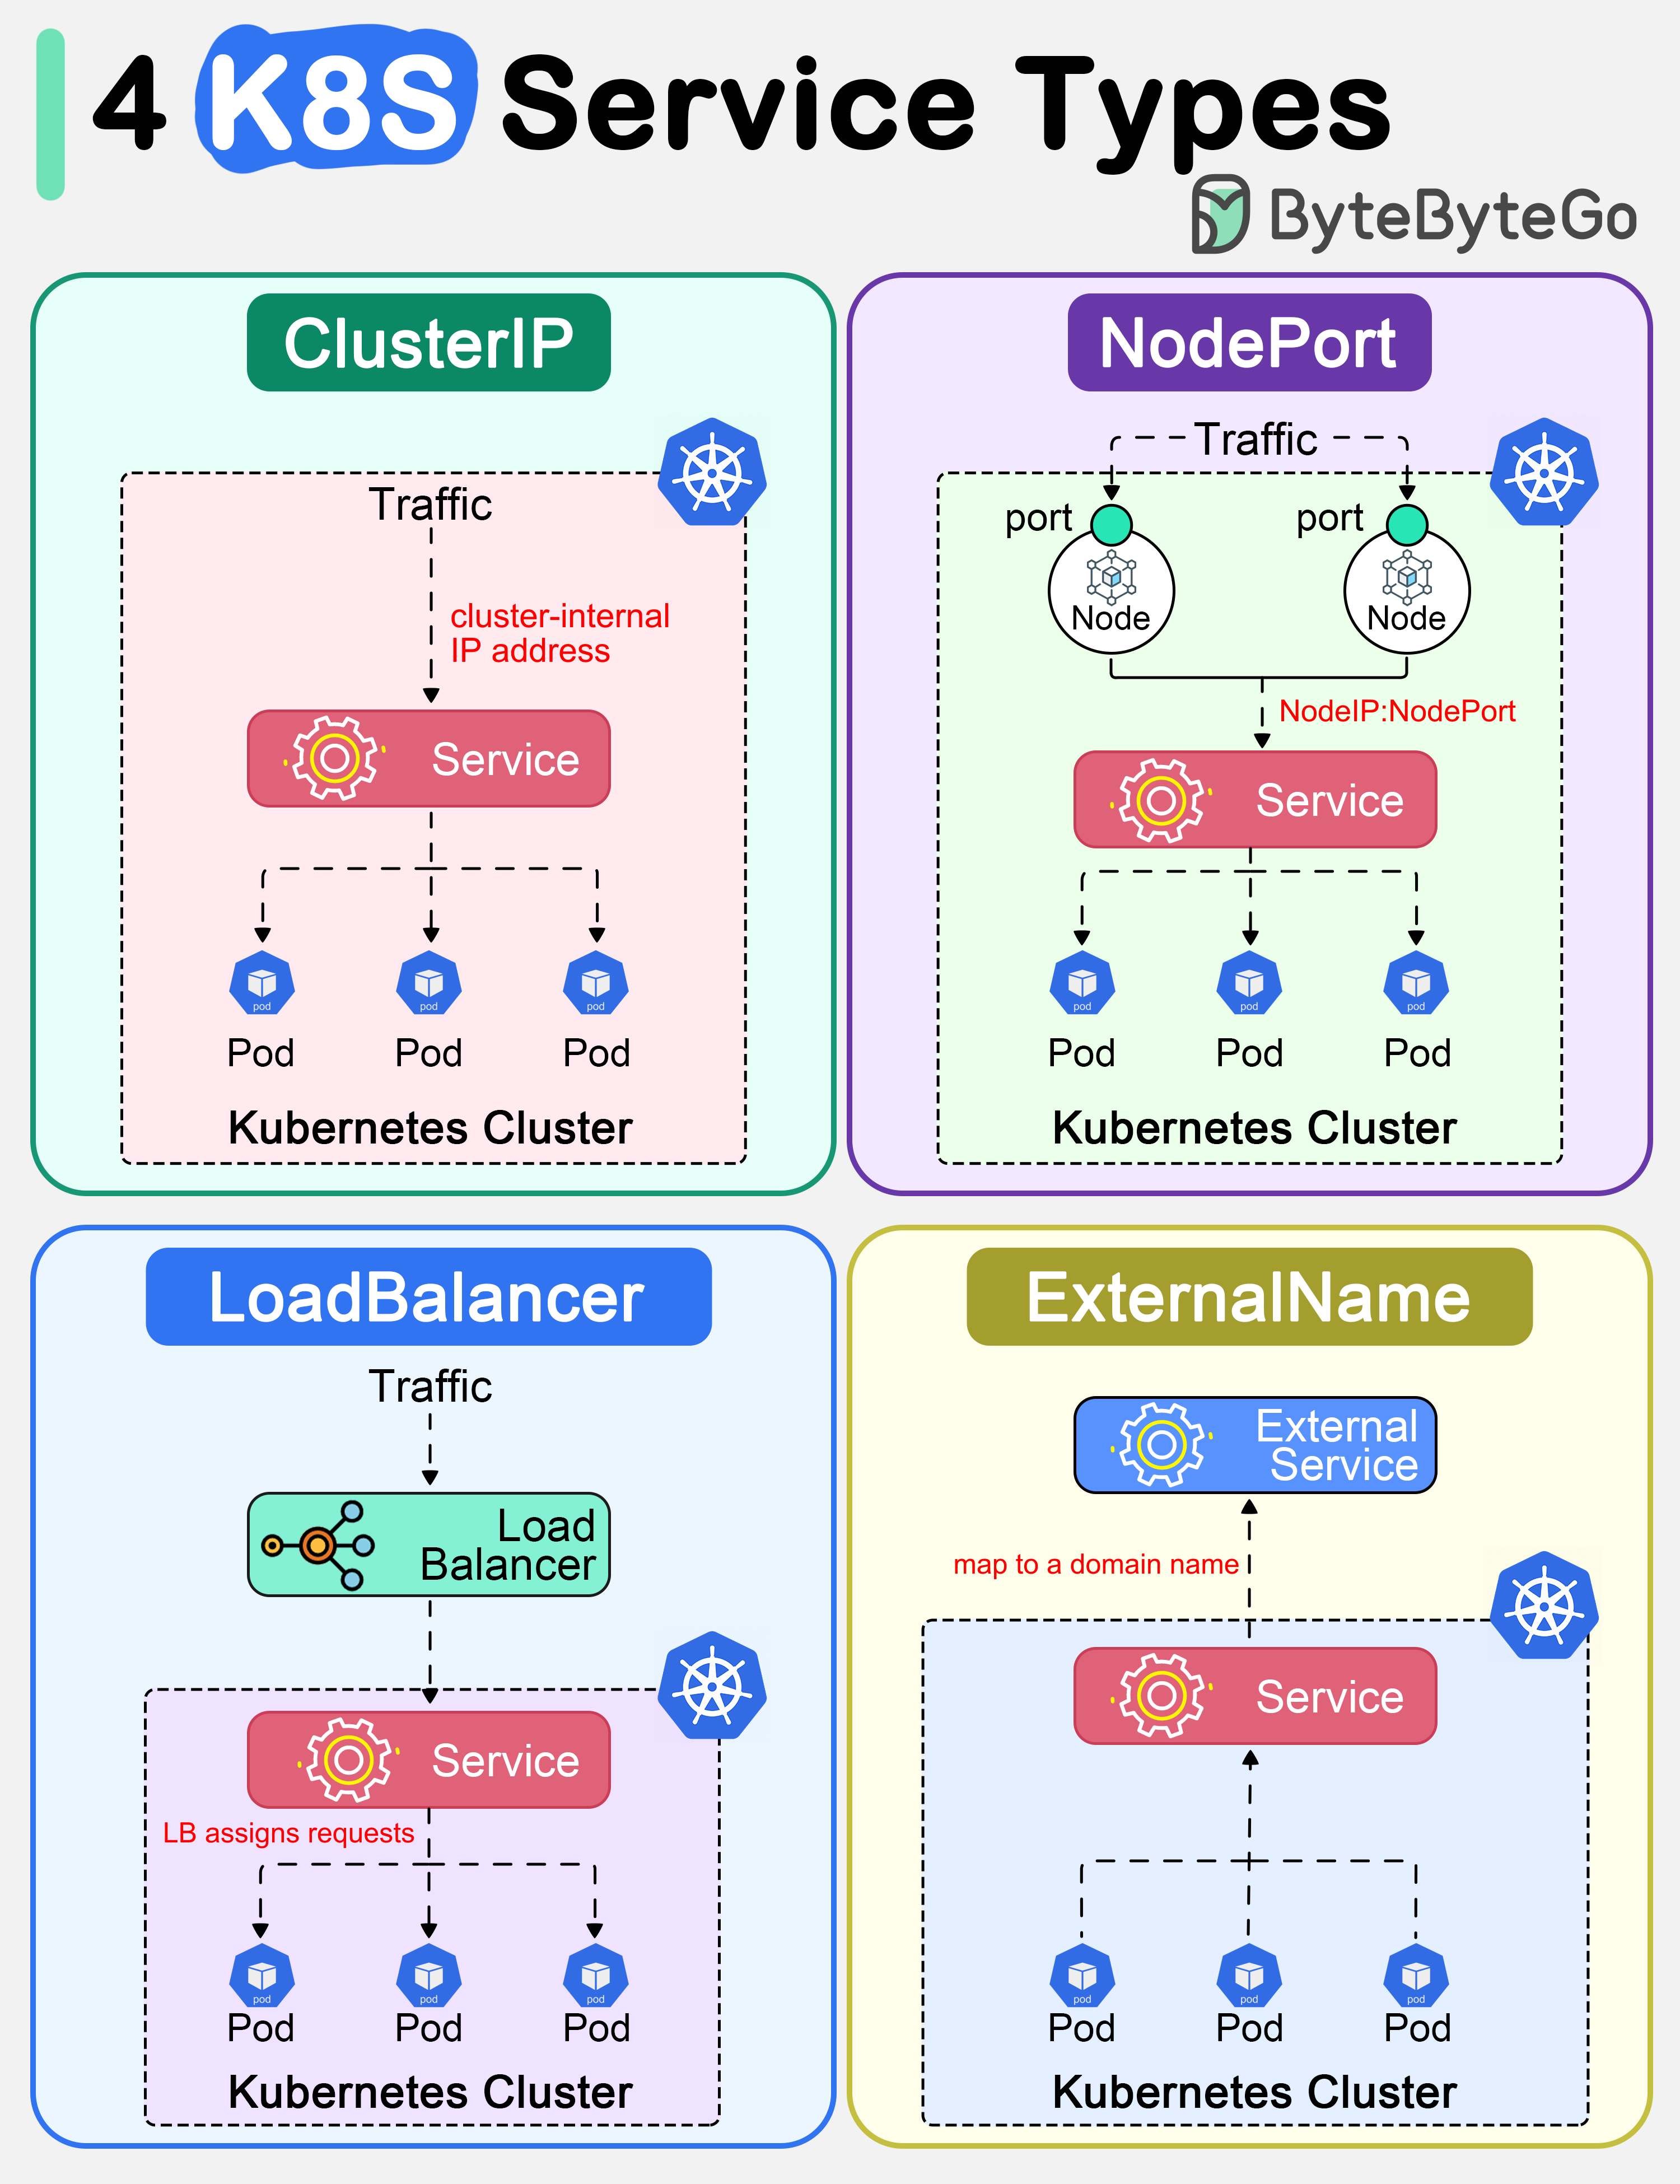
\includegraphics[width=0.85\textwidth]{figures/k8s-service-types.png}
	\caption{Types de services Kubernetes}
\end{figure}

\subparagraph{ClusterIP}
Il s’agit du type de service par défaut. Il crée une IP virtuelle interne au cluster, accessible uniquement depuis les autres composants Kubernetes. Le routage est effectué via le composant \texttt{kube-proxy}, qui configure des règles \texttt{iptables} ou \texttt{IPVS} selon la configuration du cluster.

\subparagraph{NodePort}
Ce type expose le service sur un port statique (généralement entre 30000 et 32767) sur toutes les interfaces réseau de chaque nœud. Le trafic externe accède alors aux pods via l’adresse IP d’un nœud et le port attribué.

\subparagraph{LoadBalancer}
Ce type s’appuie sur l’intégration avec un fournisseur de cloud pour provisionner automatiquement un équilibreur de charge (load balancer) et attribuer une IP publique. Il est idéal pour l’exposer à Internet, mais dépend de l’environnement cloud.

\subparagraph{ExternalName}
Ce type ne crée pas réellement de proxy mais agit comme une redirection DNS. Il permet d’exposer un service interne vers une ressource externe en mappant son nom à un domaine DNS externe, sans gestion de pods ou endpoints.

\subparagraph{Ingress}
En complément des services, l’objet \texttt{Ingress} permet de définir des règles de routage HTTP(S) avancées :
\begin{itemize}
	\item Routage basé sur les hôtes ou les chemins.
	\item Terminaison TLS.
	\item Redirections, en-têtes personnalisés, sécurité.
\end{itemize}
Un contrôleur d’Ingress (comme NGINX ou Traefik) est requis pour appliquer ces règles.

\bigskip

\subparagraph{Tableau récapitulatif des types de services Kubernetes}

\begin{longtable}{|p{4cm}|p{5cm}|p{6cm}|}
	\caption{\it{Comparatif des types de services Kubernetes}}
	\label{tab:services_k8s}                                                                                                                      \\ \hline
	\textbf{Type de service} & \textbf{Accessibilité}                  & \textbf{Utilisation typique}                                             \\ \hline
	\endfirsthead
	\multicolumn{3}{l}{\tablename\ \thetable\ -- \textit{Suite}}                                                                                  \\ \hline
	\textbf{Type de service} & \textbf{Accessibilité}                  & \textbf{Utilisation typique}                                             \\ \hline
	\endhead
	\hline \multicolumn{3}{r}{\textit{Suite de la page précédente}}                                                                               \\ \hline
	\endfoot
	\hline
	\endlastfoot

	\texttt{ClusterIP}       & Interne au cluster uniquement           & Communication entre pods ou services backend internes                    \\ \hline
	\texttt{NodePort}        & Accès via IP du nœud et port externe    & Test local, accès direct sans load balancer                              \\ \hline
	\texttt{LoadBalancer}    & IP publique attribuée automatiquement   & Exposition publique dans un environnement cloud                          \\ \hline
	\texttt{ExternalName}    & Redirection DNS vers un service externe & Connexion à des services externes (API tierces, bases de données gérées) \\ \hline

\end{longtable}
Le tableau \ref{tab:services_k8s} présente une comparaison synthétique des différents types de services proposés par Kubernetes.

\paragraph{Network Policies}

Pour renforcer la sécurité, Kubernetes propose les \texttt{NetworkPolicies}, qui définissent des règles de filtrage des flux entre pods :
\begin{itemize}
	\item Sélection des pods sources et destinations.
	\item Protocoles et ports autorisés.
	\item Isolation stricte par namespace ou par label.
\end{itemize}
Les politiques réseau nécessitent un CNI compatible (par exemple Calico).

\paragraph{DNS interne}

Kubernetes fournit un service DNS interne (CoreDNS) qui résout les noms des services et pods :
\begin{itemize}
	\item Chaque service est accessible via un nom DNS du type \texttt{myservice.mynamespace.svc.cluster.local}.
	\item Les applications peuvent utiliser la découverte de services sans configuration externe.
\end{itemize}

En combinant ces composants, le réseau Kubernetes offre un modèle cohérent, flexible et extensible qui facilite le déploiement d’applications distribuées tout en garantissant la sécurité et l’évolutivité.

\subsection{MetalLB}

MetalLB est une solution de load balancing spécialement conçue pour les clusters Kubernetes déployés en environnement on-premise. Contrairement aux plateformes cloud qui fournissent des services d’équilibrage de charge natifs, les installations locales de Kubernetes ne disposent pas par défaut d’un mécanisme équivalent pour l’attribution d’adresses IP publiques et la distribution du trafic.

\paragraph{Principales fonctionnalités}

MetalLB apporte plusieurs fonctionnalités essentielles :
\begin{itemize}
	\item \textbf{Attribution d’adresses IP virtuelles} : il permet de réserver et d’annoncer des plages d’adresses IP utilisables pour exposer les services en mode \emph{LoadBalancer}.
	\item \textbf{Distribution du trafic réseau} : il redirige les requêtes entrantes vers les pods cibles, en fonction de la configuration et de l’algorithme de balancing choisi.
	\item \textbf{Compatibilité BGP et L2} : MetalLB propose deux modes de fonctionnement :
	      \begin{itemize}
		      \item Le mode \textbf{Layer 2}, qui utilise ARP ou NDP pour annoncer l’adresse IP sur le réseau local.
		      \item Le mode \textbf{BGP}, qui permet d’établir des sessions de routage dynamique avec les routeurs de l’infrastructure.
	      \end{itemize}
\end{itemize}

\paragraph{Mécanisme de haute disponibilité (HA)}

MetalLB met en œuvre un mécanisme de haute disponibilité pour garantir la continuité de service même en cas de défaillance d’un nœud.

Dans le mode Layer 2 :
\begin{itemize}
	\item Un seul nœud dans le cluster est désigné comme \emph{speaker} pour une adresse IP donnée.
	\item En cas de panne ou d’indisponibilité du nœud speaker, les autres nœuds organisent une élection pour élire un nouveau speaker, qui prendra le relais et continuera à annoncer l’IP virtuelle sur le réseau.
\end{itemize}

Ce mécanisme permet de garantir que les services exposés restent accessibles même en cas de panne matérielle ou logicielle sur un nœud.

\paragraph{Avantages et inconvénients}

\begin{itemize}
	\item \textbf{Avantages} :
	      \begin{itemize}
		      \item Permet l’utilisation de services \texttt{LoadBalancer} en on-premise sans équipement physique supplémentaire.
		      \item Haute disponibilité grâce à la redondance des speakers.
		      \item Facilement intégrable dans un cluster Kubernetes existant.
		      \item Compatible avec les politiques réseau Kubernetes.
	      \end{itemize}

	\item \textbf{Inconvénients / Limites} :
	      \begin{itemize}
		      \item \textbf{Goulot d’étranglement potentiel} : seul le speaker actif reçoit le trafic entrant pour une IP donnée, ce qui peut limiter le débit réseau.
		      \item Ce modèle peut réduire le \emph{throughput} maximal, car le speaker redistribue ensuite le trafic vers les pods cibles situés éventuellement sur d'autres nœuds.
		      \item Le modèle ne permet pas un load balancing L4 actif/actif entre nœuds (sauf en mode BGP multi-routeur).
	      \end{itemize}
\end{itemize}

\paragraph{Remarque sur les performances}

Dans la majorité des cas d’usage (web APIs, services métiers), la limite du throughput au niveau du speaker est acceptable. En effet, le facteur limitant n’est pas la capacité réseau brute mais le temps de traitement des requêtes applicatives. Grâce au modèle distribué de Kubernetes, ce traitement est réparti entre les pods, ce qui permet de maintenir de bonnes performances globales même si un seul nœud reçoit initialement le trafic.

\begin{figure}[H]
	\centering
	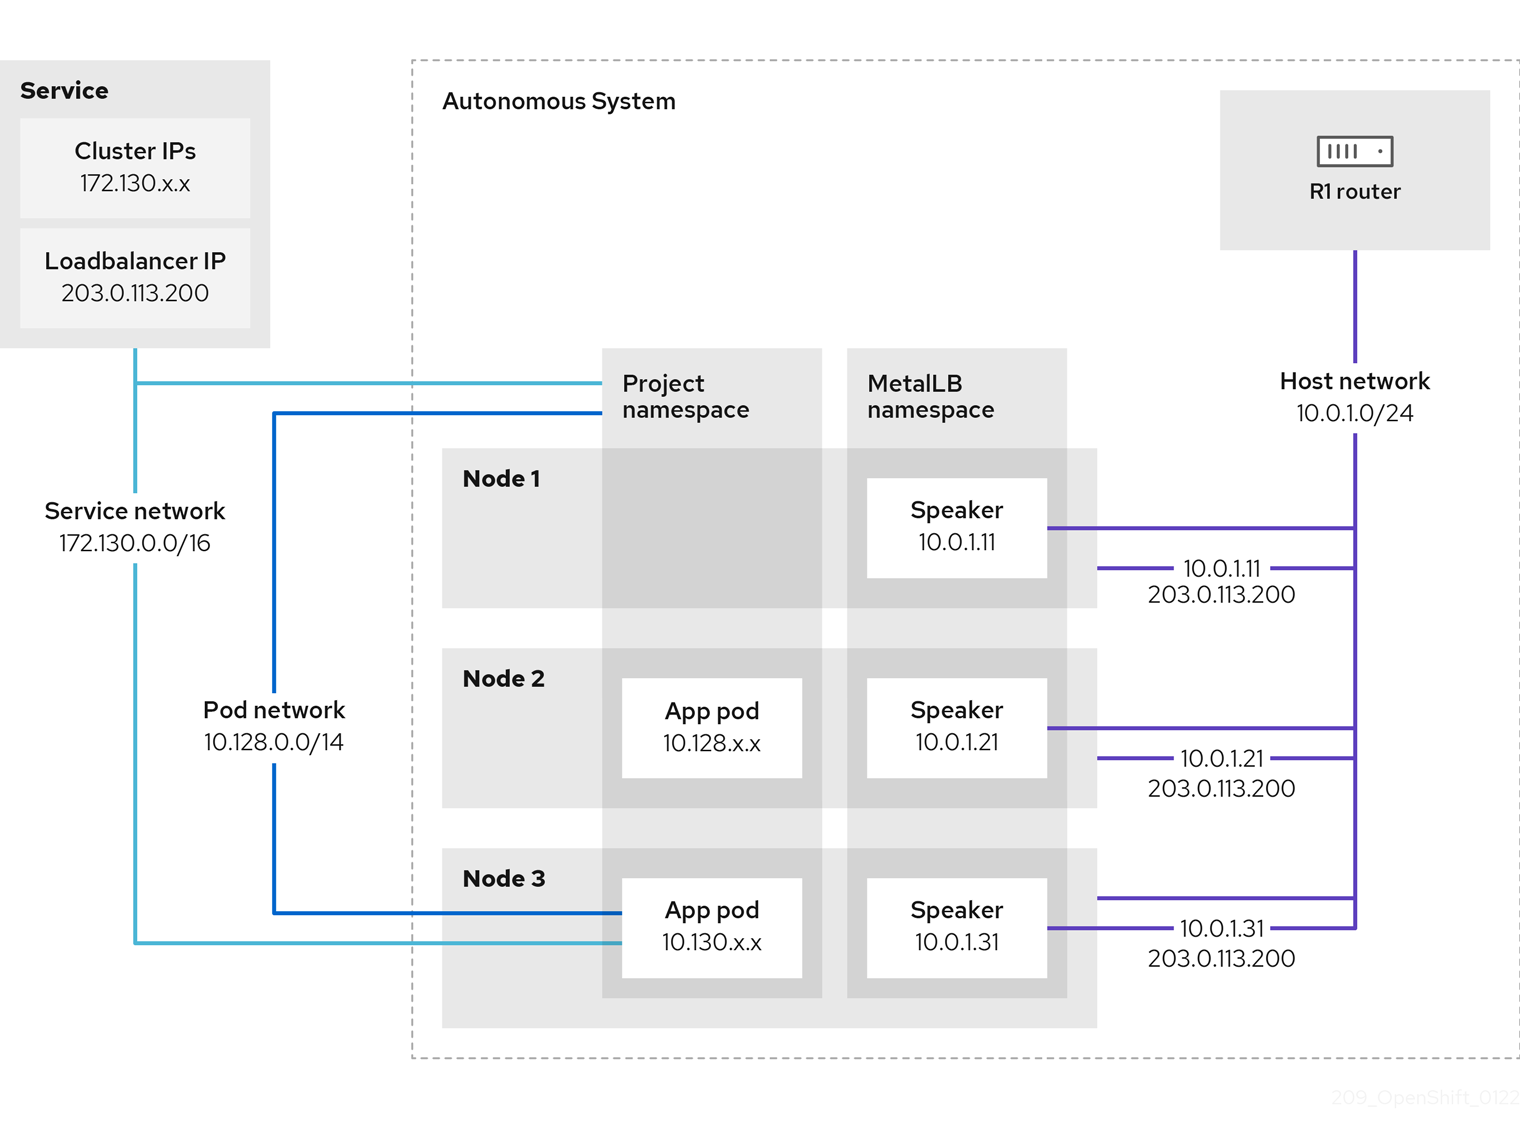
\includegraphics[width=0.85\textwidth]{figures/Metallb network.png}
	\caption{Réseau de MetalLB}
\end{figure}

\section{Mise en place des services de réseau}

Cette partie décrit la mise en œuvre et l’automatisation des services essentiels au bon fonctionnement du réseau et à la sécurisation des flux. Ces services incluent le pare-feu, le reverse proxy ainsi que la gestion centralisée des secrets.

\subsection{Configuration automatique de pfSense avec Ansible}

Le pare-feu pfSense constitue le point d’entrée et de filtrage du trafic réseau. Afin de garantir la reproductibilité de sa configuration et d’éviter les erreurs manuelles, Ansible a été utilisé pour automatiser son déploiement et sa configuration.

Pour cela, des modules spécifiques à pfSense et des collections Ansible dédiées ont été mis en œuvre, permettant notamment :
\begin{itemize}
	\item La définition des règles de filtrage (firewall rules) par groupe et par interface.
	\item La configuration des interfaces réseau et des VLANs.
	\item L’activation et la configuration du service DHCP.
	\item La gestion des utilisateurs et des certificats.
\end{itemize}

Grâce à cette approche, il est possible de versionner les configurations pfSense dans un dépôt Git et de les appliquer de manière cohérente sur plusieurs environnements.
En cas de restauration après sinistre, la remise en service peut ainsi être réalisée rapidement et de façon fiable.

\subsection{Configuration de NGINX avec Ansible}

NGINX joue un rôle central comme reverse proxy et point d’entrée HTTP(S) des applications.
La configuration de NGINX a été automatisée avec Ansible afin de :
\begin{itemize}
	\item Créer et gérer les fichiers de configuration des sites virtuels (server blocks).
	\item Générer automatiquement les certificats TLS via Let’s Encrypt.
	\item Mettre en place les règles de redirection et de réécriture des URLs.
	\item Définir les paramètres de sécurité (headers HTTP, limitation de débit).
\end{itemize}

Les rôles Ansible développés permettent de paramétrer NGINX de manière déclarative en fonction des variables d’inventaire et de secrets provenant de Vault.
Chaque modification de configuration est ainsi versionnée et peut être appliquée de façon idempotente.

\subsection{Usage de Vault pour la gestion des secrets}

La gestion centralisée et sécurisée des secrets est assurée par HashiCorp Vault.
Vault est utilisé comme source unique de vérité pour stocker et distribuer :
\begin{itemize}
	\item Les mots de passe d’accès aux services.
	\item Les clés API nécessaires aux applications.
	\item Les certificats TLS privés.
	\item Les tokens d’authentification.
\end{itemize}

L’authentification des systèmes à Vault s’effectue via AppRole et tokens dynamiques, ce qui limite le risque de compromission en cas de fuite d’identifiants.
Ansible est configuré pour interroger Vault à l’exécution des playbooks et récupérer les secrets de manière transparente.
Cette approche présente plusieurs avantages :
\begin{itemize}
	\item Les secrets ne sont jamais stockés en clair dans les dépôts Git.
	\item La rotation régulière est facilitée.
	\item Les accès sont tracés et audités.
\end{itemize}

L’intégration de Vault avec Terraform et Ansible permet ainsi de garantir un niveau de sécurité élevé tout au long du cycle de vie des environnements.

\section{Synthèse}

La combinaison d’outils tels que Proxmox, Terraform, Ansible, Vault et pfSense a permis de construire une infrastructure automatisée, sécurisée et reproductible. Cette approche s’inscrit dans la démarche Infrastructure as Code, garantissant un haut niveau de cohérence et facilitant les évolutions futures.

\section{Presentation des outils GitOps}
\subsection{Argo CD}

Argo CD est un outil open source de déploiement continu (CD) natif Kubernetes, conçu pour mettre en œuvre les pratiques GitOps. Il permet de synchroniser l’état désiré des applications, défini dans un dépôt Git, avec l’état effectif du cluster Kubernetes. En automatisant la gestion et le déploiement des manifestes, Argo CD apporte cohérence, traçabilité et résilience aux environnements cloud-native.

%point de vue metier
Argo CD répond à plusieurs enjeux stratégiques  : fiabiliser les déploiements, réduire le temps de mise en production, renforcer la traçabilité et limiter les erreurs humaines. Il offre un modèle déclaratif et auditable, conforme aux exigences de sécurité et de conformité des organisations modernes. En industrialisant le GitOps, Argo CD contribue à accélérer l’innovation tout en garantissant la stabilité des systèmes.

%point de vue logique et technique
, Argo CD s’appuie sur plusieurs composants clés  :
\begin{itemize}
	\item \textbf{Le dépôt Git}  : source unique de vérité contenant les manifestes Kubernetes (YAML) ou les définitions Kustomize/Helm.
	\item \textbf{Le contrôleur Argo CD}  : composant qui surveille les différences entre l’état souhaité (Git) et l’état réel du cluster.
	\item \textbf{L’API Server et l’interface Web}  : couche d’administration et de visualisation centralisée des applications et des synchronisations.
	\item \textbf{Les applications}  : objets Kubernetes représentant l’état désiré d’un ensemble de ressources.
	\item \textbf{Les stratégies de synchronisation}  : modes automatique ou manuel permettant de contrôler les mises à jour.
\end{itemize}

Argo CD offre un modèle de sécurité avancé, intégrant la gestion fine des permissions (RBAC), le support du SSO (OAuth2, OIDC), le chiffrement des secrets et des validations automatiques des changements.

\textbf{Exemples et cas d’usage} :
\begin{itemize}
	\item Déployer automatiquement une application Helm versionnée depuis un dépôt Git centralisé.
	\item Gérer des environnements multiples (dev, staging, production) avec des dossiers ou des branches distinctes.
	\item Appliquer des politiques de synchronisation automatique avec validation de signature Git.
	\item Visualiser les différences entre l’état courant et l’état cible et lancer un déploiement manuel.
	\item Auditer l’historique des déploiements et des changements appliqués au cluster.
\end{itemize}

\textbf{Avantages principaux} :
\begin{itemize}
	\item Mise en œuvre native du GitOps et centralisation de la configuration déclarative.
	\item Traçabilité et auditabilité complètes des changements.
	\item Intégration fluide avec Helm, Kustomize, Jsonnet et plain YAML.
	\item Réduction du risque d’erreurs grâce au contrôle automatique des dérives d’état.
	\item Interface Web ergonomique et API REST.
	\item Sécurité renforcée avec RBAC et chiffrement des secrets.
\end{itemize}

En synthèse, Argo CD est une solution stratégique pour l’automatisation et la fiabilisation des déploiements Kubernetes. Il contribue à instaurer des workflows GitOps robustes, cohérents et évolutifs, adaptés aux exigences opérationnelles des entreprises modernes.

\textbf{Références suggérées} :
\begin{itemize}
	\item Argo CD Documentation – \url{https://argo-cd.readthedocs.io/}
	\item Argo CD GitHub Repository – \url{https://github.com/argoproj/argo-cd}
	\item GitOps Principles – \url{https://www.gitops.tech/}
	\item CNCF Argo Project – \url{https://www.cncf.io/projects/argo/}
	\item Helm Documentation – \url{https://helm.sh/docs/}
\end{itemize}

\subsection{Helm}

Helm est un gestionnaire de packages Kubernetes qui permet de décrire des applications sous forme de charts. Chaque chart contient des modèles de manifestes et des fichiers de valeurs qui définissent les paramètres de l’application. Helm est particulièrement adapté lorsque :
\begin{itemize}
	\item Les applications déployées nécessitent de nombreuses options configurables.
	\item Il est souhaité de réutiliser des packages officiels ou communautaires (par exemple nginx, prometheus).
	\item Les équipes ont besoin de versionner et de publier des applications sous forme de packages standardisés.
\end{itemize}
\textbf{Exemples de cas d’usage} :
\begin{itemize}
	\item Déploiement d’un cluster Prometheus avec des paramètres personnalisés.
	\item Installation d’un Ingress Controller en adaptant les valeurs selon l’environnement.
\end{itemize}
\textbf{Exécution} : Lorsqu’Argo CD synchronise une application déclarée comme Helm dans le dépôt Git, il exécute le rendu du chart (commande helm template) avant d’appliquer les ressources générées dans le cluster.

\subsection{Kustomize}

Kustomize est un outil natif Kubernetes de composition et de personnalisation des manifestes YAML. Il fonctionne en surchargeant des ressources de base avec des patches et des overlays. Kustomize est adapté lorsque :
\begin{itemize}
	\item L’application ne nécessite pas un système de packaging complet.
	\item Les environnements (dev, recette, prod) partagent une base commune mais nécessitent des ajustements ciblés.
	\item Il est important de conserver des manifestes Kubernetes purs et lisibles.
\end{itemize}
\textbf{Exemples de cas d’usage} :
\begin{itemize}
	\item Appliquer des replicas différents selon l’environnement.
	\item Modifier les variables d’environnement ou les annotations.
\end{itemize}
\textbf{Exécution} : Argo CD supporte nativement Kustomize. Lors de la synchronisation, le contrôleur applique kustomize build pour générer les manifestes avant de les appliquer au cluster.

\paragraph{Intégration avec Argo CD}

Argo CD offre un support natif pour Helm et Kustomize. Lors de la définition d’une application, il suffit de préciser le type de source (Helm, Kustomize ou Directory). Le processus de rendu est alors entièrement automatisé :
\begin{itemize}
	\item Le contrôleur Argo CD surveille le dépôt Git et détecte les modifications.
	\item Il exécute le rendu des manifestes via Helm ou Kustomize.
	\item Les ressources générées sont comparées à l’état courant du cluster.
	\item Les différences sont appliquées automatiquement ou manuellement selon la stratégie choisie.
\end{itemize}

\paragraph{Bénéfices principaux}

Le recours à Helm et Kustomize apporte plusieurs avantages :
\begin{itemize}
	\item Réduction de la duplication des manifestes entre environnements.
	\item Simplification de la gestion des configurations dynamiques.
	\item Meilleure lisibilité et maintenabilité des définitions Kubernetes.
	\item Standardisation des déploiements grâce aux charts officiels ou internes.
\end{itemize}

\section{Mise en œuvre du modèle GitOps}

Le modèle GitOps vise à centraliser la définition de l’infrastructure et des applications dans des dépôts Git versionnés, en s’appuyant sur un opérateur qui applique automatiquement l’état souhaité dans le cluster Kubernetes.
Dans ce projet, l’outil \textbf{Argo CD} a été retenu pour assurer ce rôle.
La démarche GitOps permet d’améliorer la traçabilité, la cohérence et l’automatisation des déploiements.

\subsection{Préparation des manifestes des outils internes}

Avant l’installation d’Argo CD, les manifestes Kubernetes décrivant les composants internes nécessaires au bon fonctionnement de la plateforme ont été préparés.
Ces manifestes incluent :
\begin{itemize}
	\item Les configurations des namespaces réservés (par exemple \texttt{argocd}, \texttt{monitoring}, \texttt{tools}).
	\item Les déploiements de services annexes tels que les opérateurs de sauvegarde et les contrôleurs réseau.
	\item Les configurations des ressources communes (ConfigMaps, Secrets, RBAC).
\end{itemize}

L’ensemble de ces manifestes est versionné dans un dépôt Git dédié à l’infrastructure, garantissant une source unique de vérité et la possibilité de reconstruire intégralement l’environnement.

\subsection{Installation d’Argo CD}

L’installation d’Argo CD a été réalisée via l’application des manifestes officiels fournis par le projet.
Le processus s’effectue en deux étapes principales :
\begin{itemize}
	\item Création du namespace dédié (\texttt{argocd}).
	\item Application du manifest d’installation complet :
	      \begin{verbatim}
kubectl apply -n argocd -f https://raw.githubusercontent.com/argoproj/argo-cd/stable/manifests/install.yaml
\end{verbatim}
\end{itemize}

Après l’installation, les pods principaux (API server, repo server, application controller et dex) sont déployés automatiquement.
L’interface web d’Argo CD permet de superviser les applications GitOps et leur état de synchronisation.

\subsection{Configuration de l’authentification}

La sécurisation de l’accès à Argo CD est essentielle.
Les mesures suivantes ont été mises en place :
\begin{itemize}
	\item (A discuter si on veut l'integrer avec SSO Keyloak) Activation de l’authentification via Dex avec un connecteur LDAP, permettant une intégration avec l’annuaire interne.
	\item Création de rôles et de policies RBAC pour définir des droits différenciés selon les équipes (lecture seule, modification, administration).
	\item Rotation automatique des tokens d’accès.
	\item Activation de TLS pour sécuriser les communications avec l’interface web.
\end{itemize}

Ces mécanismes garantissent que seuls les utilisateurs autorisés peuvent interagir avec les ressources et déclencher des déploiements.

\subsection{Configuration des synchronisations}

La synchronisation automatique entre l’état déclaré dans Git et l’état réel du cluster est un principe fondamental de GitOps.
Argo CD a été configuré avec les paramètres suivants :
\begin{itemize}
	\item Mode de synchronisation automatique (\texttt{auto-sync}) activé sur les applications critiques.
	\item Validation stricte des manifests avant application.
	\item Prise en charge des stratégies de \textit{pruning} pour supprimer les ressources obsolètes.
	\item Notification par webhook et alerting en cas d’écart détecté entre l’état souhaité et l’état courant.
\end{itemize}

Cette configuration permet de garantir que le cluster converge toujours vers l’état décrit dans les dépôts Git et de détecter les modifications manuelles non autorisées.

\subsection{Préparation des manifestes des applications développées par Oneex pour des environnements différents}

Les applications développées par Oneex ont été déployées sur plusieurs environnements (développement, recette, production).
Pour assurer la cohérence et l’adaptabilité, les manifestes Kubernetes ont été préparés selon les principes suivants :
\begin{itemize}
	\item Utilisation de \texttt{kustomize} pour générer des variantes par environnement (par exemple configuration des replicas, des ressources et des variables d’environnement).
	\item Définition de ConfigMaps et de Secrets séparés selon les contextes.
	\item Structuration des dépôts Git avec des arborescences claires par application et par environnement.
	\item Mise en place de règles de validation continue (linting et contrôle de schéma) avant validation des commits.
\end{itemize}

Cette approche permet de disposer d’un processus de déploiement uniforme, de simplifier la maintenance et de garantir que chaque environnement est conforme aux spécifications attendues.


\chapter{Intégration et livraison continues}\label{chapter:cicd}
\subsection{GitLab CI}

GitLab CI (Continuous Integration) est un système d’intégration et de livraison continues intégré nativement dans GitLab, une plateforme DevOps complète de gestion du cycle de vie applicatif. Il permet d’automatiser la construction, les tests, la validation, le packaging et le déploiement des applications en s’appuyant sur des pipelines définis de manière déclarative. GitLab CI est aujourd’hui largement utilisé dans les organisations souhaitant industrialiser leurs workflows de développement et renforcer la qualité logicielle.

 %point de vue metier
 GitLab CI répond à plusieurs enjeux stratégiques  : accélérer le time-to-market, réduire les erreurs humaines, renforcer la traçabilité des changements et améliorer la collaboration entre équipes. Grâce à sa proximité avec le dépôt Git, il apporte une cohérence totale entre le code source, l’historique des commits et les pipelines d’automatisation. Il contribue ainsi à la modernisation et à la professionnalisation des processus de développement.

 %point de vue logique et technique
, GitLab CI repose sur plusieurs concepts essentiels  :
\begin{itemize}
	\item \textbf{Le fichier \texttt{.gitlab-ci.yml}}  : fichier de configuration déclaratif placé à la racine du dépôt, qui décrit les jobs et les étapes du pipeline.
	\item \textbf{Les jobs}  : unités atomiques qui exécutent des scripts ou des commandes (build, test, deploy).
	\item \textbf{Les stages}  : regroupements logiques des jobs (par exemple, build, test, deploy) exécutés séquentiellement ou en parallèle.
	\item \textbf{Les runners}  : exécutants (machines ou conteneurs) qui traitent les jobs. Ils peuvent être partagés, spécifiques ou autoscalés.
	\item \textbf{Les variables}  : valeurs dynamiques injectées dans les pipelines (clés, secrets, paramètres d’environnement).
	\item \textbf{Les artefacts}  : fichiers générés par les jobs et transmis entre étapes.
\end{itemize}

GitLab CI prend en charge de nombreuses fonctionnalités avancées  : intégration Kubernetes, déclencheurs manuels (manual actions), pipelines multi-projets, stratégies de déploiement progressif et vérification des politiques de sécurité.

\textbf{Exemples et cas d’usage} :
\begin{itemize}
	\item Compiler automatiquement une application dès la création d’une merge request.
	\item Exécuter des tests unitaires et fonctionnels dans un pipeline parallèle.
	\item Construire et publier des images Docker sur GitLab Container Registry.
	\item Déployer des applications sur Kubernetes via Helm ou kubectl.
	\item Générer et publier automatiquement la documentation technique.
\end{itemize}

\textbf{Avantages principaux} :
\begin{itemize}
	\item Intégration native avec GitLab et l’ensemble du cycle de vie DevOps.
	\item Modèle déclaratif simple et lisible.
	\item Traçabilité et auditabilité complète des pipelines.
	\item Compatibilité avec les conteneurs et les environnements Kubernetes.
	\item Gestion sécurisée des secrets et des variables sensibles.
	\item Large écosystème de templates, exemples et intégrations communautaires.
\end{itemize}

En synthèse, GitLab CI est une solution stratégique pour automatiser l’intégration et la livraison continues. Il permet aux équipes de gagner en efficacité opérationnelle, d’améliorer la qualité logicielle et d’accélérer la mise en production des innovations.

\textbf{Références suggérées} :
\begin{itemize}
	\item GitLab CI Documentation – \url{https://docs.gitlab.com/ee/ci/}
	\item GitLab CI YAML Reference – \url{https://docs.gitlab.com/ee/ci/yaml/}
	\item GitLab Runners – \url{https://docs.gitlab.com/runner/}
	\item GitLab Kubernetes Integration – \url{https://docs.gitlab.com/ee/user/project/clusters/}
	\item GitLab Auto DevOps – \url{https://docs.gitlab.com/ee/topics/autodevops/}
\end{itemize}

\subsection{Commitlint}

Commitlint est un outil open source qui permet de vérifier que les messages de commit respectent un format prédéfini. Il est particulièrement utilisé dans les workflows Git modernes pour renforcer la cohérence des messages de commit, faciliter la génération automatique de changelogs et standardiser la documentation des évolutions logicielles. Commitlint est souvent intégré à des processus de validation automatisés grâce aux hooks Git (par exemple avec Husky) ou aux pipelines CI/CD.

 %point de vue metier
 Commitlint répond à plusieurs enjeux stratégiques  : améliorer la lisibilité de l’historique des changements, garantir une traçabilité complète des évolutions, renforcer la qualité documentaire et faciliter les audits. La standardisation des messages de commit contribue à instaurer une culture de rigueur et de professionnalisation au sein des équipes de développement.

 %point de vue logique et technique
, Commitlint s’appuie sur plusieurs concepts essentiels  :
\begin{itemize}
	\item \textbf{Les règles de validation}  : définissent le format attendu des commits (par exemple, le standard Conventional Commits).
	\item \textbf{Le parser}  : analyse le message de commit et vérifie qu’il correspond au schéma spécifié.
	\item \textbf{La configuration}  : fichier \texttt{commitlint.config.js} où l’on définit les règles, les exceptions et les presets.
	\item \textbf{L’intégration avec Husky}  : permet de déclencher la vérification lors du hook \texttt{commit-msg}.
\end{itemize}

Le standard le plus répandu est \textbf{Conventional Commits}, qui impose un format structuré  :
\begin{verbatim}
<type>(<scope>): <subject>

Exemple :
feat(auth): add JWT authentication
fix(api): handle null pointer exception
docs(readme): update installation instructions
\end{verbatim}

Ce format facilite l’automatisation des versions sémantiques (Semantic Versioning) et la génération des changelogs.

\textbf{Exemples et cas d’usage} :
\begin{itemize}
	\item Empêcher la validation d’un commit si le message ne commence pas par un type valide (ex.: feat, fix, chore).
	\item Bloquer les commits dont le titre dépasse une longueur maximale.
	\item Valider automatiquement tous les messages de commit dans un pipeline CI/CD.
	\item Générer des changelogs structurés à partir des commits normalisés.
	\item Appliquer un format de commit homogène sur plusieurs équipes et projets.
\end{itemize}

\textbf{Avantages principaux} :
\begin{itemize}
	\item Standardisation et lisibilité accrue des messages de commit.
	\item Réduction des erreurs et des incohérences documentaires.
	\item Automatisation des processus de release et de génération de changelogs.
	\item Compatibilité avec les pratiques GitOps et CI/CD.
	\item Facilité d’intégration avec Husky et d’autres outils de hooks Git.
\end{itemize}

En synthèse, Commitlint est une brique essentielle pour industrialiser et professionnaliser la gestion des versions et la documentation des projets logiciels. Il contribue à instaurer une culture DevOps rigoureuse et à améliorer la traçabilité du cycle de développement.

\textbf{Références suggérées} :
\begin{itemize}
	\item Commitlint Documentation – \url{https://commitlint.js.org/}
	\item Conventional Commits – \url{https://www.conventionalcommits.org/}
	\item Husky Documentation – \url{https://typicode.github.io/husky/}
	\item Semantic Versioning – \url{https://semver.org/}
	\item GitHub Commitlint Repository – \url{https://github.com/conventional-changelog/commitlint}
\end{itemize}


\subsection{Husky}

Husky est un outil open source permettant de gérer et d’exécuter des hooks Git de manière simple et centralisée dans les projets logiciels. Il facilite l’automatisation de tâches de validation et de mise en conformité lors des événements Git, tels que les commits, les pushs ou les merges. Grâce à sa configuration déclarative, Husky contribue à instaurer des pratiques DevOps rigoureuses et à renforcer la qualité du code tout au long du cycle de développement.

 %point de vue metier
 Husky répond à plusieurs enjeux stratégiques  : réduire les erreurs humaines, homogénéiser les workflows entre équipes, accélérer le feedback lors des validations et améliorer la traçabilité des changements. Il constitue un levier essentiel de professionnalisation, car il garantit que les standards de qualité (tests, linting, conventions de commit) sont systématiquement respectés avant d’intégrer le code au référentiel principal.

 %point de vue logique et technique
, Husky repose sur plusieurs concepts clés  :
\begin{itemize}
	\item \textbf{Les hooks Git}  : scripts déclenchés automatiquement par Git à différents moments du cycle de vie (par exemple \texttt{pre-commit}, \texttt{commit-msg}, \texttt{pre-push}).
	\item \textbf{La configuration}  : Husky utilise des commandes déclarées dans le fichier \texttt{package.json} ou dans des fichiers dédiés (\texttt{.husky/pre-commit}).
	\item \textbf{Les intégrations}  : Husky fonctionne avec de nombreux outils tels que ESLint, Prettier, Commitlint ou les tests unitaires.
	\item \textbf{Le workflow Node.js}  : bien qu’installé via npm ou Yarn, Husky est indépendant du langage utilisé dans le projet.
\end{itemize}

Les hooks les plus fréquemment utilisés sont  :
\begin{itemize}
	\item \texttt{pre-commit}  : exécute des validations avant l’enregistrement d’un commit (linting, tests).
	\item \texttt{commit-msg}  : vérifie que le message de commit respecte une convention donnée.
	\item \texttt{pre-push}  : lance des vérifications avant l’envoi du code sur le dépôt distant.
\end{itemize}

\textbf{Exemples et cas d’usage} :
\begin{itemize}
	\item Lancer ESLint automatiquement sur les fichiers modifiés avant chaque commit.
	\item Exécuter Commitlint pour garantir que les messages de commit respectent Conventional Commits.
	\item Vérifier que les tests unitaires passent avant chaque push.
	\item Appliquer Prettier pour uniformiser le formatage du code source.
	\item Bloquer la création de commits vides ou sans description.
\end{itemize}

\textbf{Avantages principaux} :
\begin{itemize}
	\item Standardisation des processus de validation dans toute l’équipe.
	\item Réduction des erreurs humaines et des régressions en amont des CI/CD.
	\item Facilité de mise en œuvre et de configuration.
	\item Compatibilité avec de nombreux outils de qualité logicielle.
	\item Exécution rapide et locale, sans dépendre de l’environnement distant.
\end{itemize}

En synthèse, Husky est un composant essentiel pour fiabiliser et automatiser les workflows de validation des projets modernes. Il contribue à instaurer une culture DevOps orientée qualité et à renforcer la cohérence entre les contributeurs.

\textbf{Références suggérées} :
\begin{itemize}
	\item Husky Documentation – \url{https://typicode.github.io/husky/}
	\item Git Hooks Documentation – \url{https://git-scm.com/docs/githooks}
	\item Commitlint Documentation – \url{https://commitlint.js.org/}
	\item ESLint Documentation – \url{https://eslint.org/docs/latest/}
	\item Prettier Documentation – \url{https://prettier.io/docs/en/}
\end{itemize}


\subsection{Semantic Release}

Semantic Release est un outil open source qui automatise le versionnement et la publication des packages logiciels en s’appuyant sur les messages de commit et le principe du versionnement sémantique (Semantic Versioning). Il supprime le besoin de mise à jour manuelle du numéro de version et de rédaction des changelogs, contribuant ainsi à la fiabilisation et à l’industrialisation des processus de release.

 %point de vue metier
 Semantic Release répond à plusieurs enjeux stratégiques  : réduire les erreurs humaines dans les versions publiées, accélérer le cycle de livraison, renforcer la traçabilité des évolutions et homogénéiser les workflows de publication entre équipes. En automatisant intégralement la release, il permet aux développeurs de se concentrer sur la qualité fonctionnelle plutôt que sur les tâches administratives.

 %point de vue logique et technique
, Semantic Release repose sur plusieurs concepts clés  :
\begin{itemize}
	\item \textbf{Les conventions de commit}  : le projet s’appuie sur des formats structurés (par exemple Conventional Commits) pour déduire automatiquement l’impact des changements (correctifs, nouvelles fonctionnalités, breaking changes).
	\item \textbf{Le calcul automatique de la version}  : en fonction des types de commits depuis la dernière release, Semantic Release incrémente la version majeure, mineure ou corrective.
	\item \textbf{La génération du changelog}  : compilation automatique des changements pertinents dans un format lisible.
	\item \textbf{La publication}  : déploiement automatisé vers les registres de packages (npm, Maven, Docker Hub) et création des tags Git correspondants.
\end{itemize}

Semantic Release s’intègre naturellement dans des pipelines CI/CD (GitHub Actions, GitLab CI, CircleCI), garantissant que chaque merge dans la branche principale déclenche la création d’une nouvelle version stable.

\textbf{Exemples et cas d’usage} :
\begin{itemize}
	\item Publier automatiquement un package npm lorsque de nouvelles fonctionnalités sont mergées.
	\item Générer un changelog détaillé à partir des commits, sans intervention manuelle.
	\item Tagger les versions dans Git et créer des releases GitHub avec les notes correspondantes.
	\item Déclencher un pipeline de build Docker et pousser l’image versionnée sur un registre.
	\item Refuser les releases en cas de non-respect des conventions de commit.
\end{itemize}

\textbf{Avantages principaux} :
\begin{itemize}
	\item Automatisation complète et fiabilisée du cycle de versionnement et de publication.
	\item Réduction drastique des erreurs humaines et des oublis dans la gestion des versions.
	\item Traçabilité et transparence accrues grâce aux changelogs générés automatiquement.
	\item Compatibilité avec de nombreux systèmes CI/CD et écosystèmes de packaging.
	\item Homogénéité des pratiques de release entre les projets et les équipes.
\end{itemize}

En synthèse, Semantic Release est une solution stratégique pour les organisations souhaitant industrialiser et sécuriser leur processus de publication. Il apporte une cohérence et une rapidité qui renforcent la qualité et la crédibilité des livraisons logicielles.

\textbf{Références suggérées} :
\begin{itemize}
	\item Semantic Release Documentation – \url{https://semantic-release.gitbook.io/}
	\item Conventional Commits – \url{https://www.conventionalcommits.org/}
	\item Semantic Versioning – \url{https://semver.org/}
	\item GitHub Actions Documentation – \url{https://docs.github.com/en/actions}
	\item npm Publishing Guide – \url{https://docs.npmjs.com/creating-and-publishing-unscoped-public-packages}
\end{itemize}

\chapter{Observabilité, supervision et audits}\label{chapter:observabilite_auditing}
\section{Introduction}

L’observabilité constitue un pilier essentiel dans la gestion moderne des systèmes distribués. Elle regroupe l’ensemble des pratiques, outils et processus permettant de comprendre le comportement d’une infrastructure, de détecter les anomalies et de garantir la conformité aux exigences de sécurité et de qualité de service.
Dans le contexte des architectures conteneurisées et des microservices, la complexité opérationnelle s’est fortement accrue. Chaque requête peut transiter par de nombreux composants, rendant le diagnostic des incidents particulièrement difficile sans outils adaptés.

De plus, les exigences réglementaires et les bonnes pratiques imposent de disposer d’audits précis des accès, des changements et des événements critiques. L’observabilité et l’audit ne se limitent donc pas à la surveillance technique, mais participent également à la gouvernance et à la gestion des risques.

\subsection{Contexte et enjeux de l'observabilité et de l'audit}

La mise en place d’un dispositif d’observabilité répond à plusieurs enjeux majeurs :

\begin{itemize}
	\item \textbf{Diagnostic rapide des incidents} : être capable de reconstituer le scénario précis ayant conduit à une panne ou à un comportement inattendu.
	\item \textbf{Optimisation des performances} : mesurer et analyser les temps de réponse, l’utilisation des ressources et la saturation éventuelle des composants.
	\item \textbf{Sécurité et traçabilité} : enregistrer les accès, les tentatives d’intrusion et les changements de configuration, afin de disposer de preuves en cas d’incident de sécurité.
	\item \textbf{Conformité réglementaire} : répondre aux obligations légales ou contractuelles en matière de conservation des journaux et de traçabilité des actions (par exemple, RGPD, ISO 27001).
	\item \textbf{Amélioration continue} : exploiter les données collectées pour identifier les points faibles et guider les évolutions de l’architecture.
\end{itemize}

Dans le cadre de ce projet, l’objectif est de fournir une visibilité unifiée sur l’état de l’infrastructure Kubernetes, des services applicatifs et des flux réseau, en s’appuyant sur des outils open source et des processus automatisés.

\section{État de l'art et tendances actuelles}

L’état de l’art de l’observabilité se structure autour de trois piliers principaux, souvent désignés sous l’acronyme \textbf{MELT} (Metrics, Events, Logs, Traces) :

\begin{enumerate}
	\item \textbf{Les métriques} : valeurs numériques collectées à intervalles réguliers (CPU, mémoire, latence). Des solutions comme Prometheus ou InfluxDB permettent de stocker et d’interroger ces mesures.
	\item \textbf{Les événements et alertes} : notifications déclenchées par un seuil ou un changement d’état. Ces événements sont souvent gérés par Alertmanager ou des systèmes de gestion d’incidents (PagerDuty, Opsgenie).
	\item \textbf{Les logs} : traces textuelles produites par les applications et les composants système. Les solutions modernes (Elastic Stack, Loki) facilitent la collecte et la recherche en temps réel.
	\item \textbf{Les traces distribuées} : enregistrements du parcours d’une requête à travers les microservices. Des outils comme Jaeger et OpenTelemetry sont devenus des standards de facto.
\end{enumerate}

Les tendances actuelles mettent en avant plusieurs évolutions :

\begin{itemize}
	\item \textbf{L’adoption massive de l’open source} : la plupart des organisations privilégient des solutions libres et communautaires pour éviter l’enfermement propriétaire.
	\item \textbf{Le modèle as-a-Service} : de nombreux acteurs (Datadog, New Relic, Grafana Cloud) proposent des plateformes hébergées intégrant l’ensemble des fonctionnalités d’observabilité.
	\item \textbf{La convergence des données} : les métriques, logs et traces ne sont plus traités isolément mais regroupés dans des plateformes unifiées facilitant les corrélations.
	\item \textbf{L’intégration avec GitOps et l’automatisation} : les configurations de monitoring et d’alerting sont versionnées et déployées de la même manière que les ressources Kubernetes.
	\item \textbf{La montée en puissance d’OpenTelemetry} : ce projet CNCF s’impose comme le standard unique de collecte de la télémétrie dans les environnements cloud-native.
\end{itemize}

Ces évolutions permettent de construire des systèmes plus résilients, plus sécurisés et plus faciles à maintenir, tout en apportant une meilleure compréhension globale des environnements complexes.

\subsection{Grafana}

Grafana est une solution open source de visualisation et d’exploration de données, largement utilisée pour la supervision des infrastructures, le monitoring applicatif et l’analyse d’indicateurs métiers. Elle permet de créer des tableaux de bord interactifs et personnalisables qui agrègent des données provenant de multiples sources (Prometheus, InfluxDB, Elasticsearch, Loki, MySQL, etc.). Grâce à son approche modulaire et à sa richesse fonctionnelle, Grafana s’est imposé comme un standard de facto dans l’écosystème cloud-native et DevOps.

%point de vue metier
Grafana répond à plusieurs enjeux stratégiques  : renforcer la visibilité sur les systèmes critiques, réduire le temps de résolution des incidents, et améliorer la qualité des services. En centralisant la visualisation et l’analyse des métriques, logs et traces, Grafana facilite la prise de décision et contribue à l’amélioration continue des processus opérationnels. Son interface conviviale et ses capacités de partage simplifient la collaboration entre équipes techniques et parties prenantes.

%point de vue logique et technique
, Grafana repose sur plusieurs composants essentiels  :
\begin{itemize}
	\item \textbf{Les datasources}  : connecteurs vers des bases de données et des systèmes de monitoring (Prometheus, Graphite, ElasticSearch, CloudWatch, etc.).
	\item \textbf{Les dashboards}  : ensembles de panels configurables qui visualisent les données sous forme de graphiques, jauges, tableaux et alertes.
	\item \textbf{Les panels}  : éléments de visualisation individuels, paramétrés avec des requêtes, des transformations et des styles personnalisés.
	\item \textbf{Les alertes}  : règles qui surveillent les seuils définis et déclenchent des notifications en cas d’anomalie.
	\item \textbf{Les organisations et utilisateurs}  : système de gestion des accès, des permissions et des partages.
\end{itemize}

Grafana peut être déployé en standalone ou intégré dans des stacks d’observabilité complètes (exemple  : Prometheus + Loki + Grafana). Son API REST et son support des plugins en font un outil particulièrement extensible et adaptable à tous les cas d’usage.

\textbf{Exemples et cas d’usage} :
\begin{itemize}
	\item Visualiser en temps réel les métriques d’un cluster Kubernetes (CPU, mémoire, pods, etc.) en s’appuyant sur Prometheus.
	\item Corréler les logs applicatifs via Loki avec les indicateurs de performance pour diagnostiquer plus rapidement un incident.
	\item Configurer des alertes pour notifier les équipes DevOps en cas de dépassement d’un seuil critique (ex. latence élevée).
	\item Créer des tableaux de bord métiers synthétiques avec des indicateurs clés (KPI) accessibles aux décideurs.
	\item Intégrer Grafana avec Slack ou PagerDuty pour centraliser les alertes et les escalades.
\end{itemize}

\textbf{Avantages principaux} :
\begin{itemize}
	\item Plateforme unifiée de visualisation multi-sources et multi-formats.
	\item Interface ergonomique et hautement personnalisable.
	\item Large écosystème de plugins, dashboards communautaires et connecteurs.
	\item Support des alertes natives et intégration avec les systèmes de notification.
	\item Extensibilité via API REST, provisioning as code et gestion des permissions fine.
	\item Solution open source mature, supportée par une large communauté.
\end{itemize}

En synthèse, Grafana est une brique centrale des stratégies d’observabilité modernes. Il permet aux organisations de transformer leurs données en connaissances actionnables, d’améliorer la performance opérationnelle et de renforcer la confiance dans les systèmes distribués.

\textbf{Références suggérées} :
\begin{itemize}
	\item Grafana Documentation – \url{https://grafana.com/docs/}
	\item Grafana GitHub Repository – \url{https://github.com/grafana/grafana}
	\item Prometheus Documentation – \url{https://prometheus.io/docs/}
	\item Loki Documentation – \url{https://grafana.com/docs/loki/latest/}
	\item Grafana Labs Blog – \url{https://grafana.com/blog/}
\end{itemize}

\subsection{Prometheus}

Prometheus est une solution open source de monitoring et d’alerte initialement développée par SoundCloud, puis incubée par la Cloud Native Computing Foundation (CNCF). Il est devenu l’un des piliers des architectures cloud-native grâce à sa capacité à collecter, stocker et interroger des métriques temporelles de manière performante. Prometheus est particulièrement reconnu pour son modèle de données multidimensionnel, son langage de requête puissant (PromQL) et sa facilité d’intégration avec Kubernetes.

%point de vue metier
Prometheus répond à plusieurs enjeux essentiels  : renforcer la visibilité sur les systèmes critiques, anticiper les incidents par une surveillance proactive et réduire le temps moyen de résolution des problèmes (MTTR). Il contribue à l’amélioration continue des performances applicatives et à la qualité de service délivrée aux utilisateurs. Grâce à sa modularité, Prometheus s’adapte à des environnements variés (infrastructures cloud, conteneurs, clusters Kubernetes, applications legacy).

%point de vue logique et technique
, Prometheus repose sur plusieurs composants clés  :
\begin{itemize}
	\item \textbf{Le serveur Prometheus}  : responsable de la collecte des métriques via le protocole HTTP/HTTPS (pull model) et du stockage local des séries temporelles.
	\item \textbf{Les exporters}  : processus ou agents qui exposent des métriques au format Prometheus (ex.: Node Exporter, Blackbox Exporter, MySQL Exporter).
	\item \textbf{Le langage PromQL}  : langage de requête permettant d’agréger, filtrer et analyser les métriques.
	\item \textbf{Les règles d’alerte}  : expressions PromQL évaluées en continu pour générer des alertes.
	\item \textbf{Alertmanager}  : composant dédié à la gestion et au routage des alertes vers les canaux de notification (email, Slack, PagerDuty).
\end{itemize}

Prometheus est particulièrement bien intégré dans l’écosystème Kubernetes grâce à la découverte de services automatique, facilitant ainsi la supervision des clusters et des workloads dynamiques.

\textbf{Exemples et cas d’usage} :
\begin{itemize}
	\item Superviser l’utilisation CPU et mémoire des nœuds Kubernetes via Node Exporter.
	\item Mesurer la latence et le taux d’erreurs des endpoints HTTP exposés par des microservices.
	\item Définir une alerte déclenchée lorsque la disponibilité d’un service passe sous un seuil critique.
	\item Stocker des métriques de performance applicative pour des analyses historiques.
	\item Visualiser les métriques dans Grafana grâce au connecteur natif Prometheus.
\end{itemize}

\textbf{Avantages principaux} :
\begin{itemize}
	\item Modèle de collecte pull simplifiant l’intégration avec les workloads dynamiques.
	\item Stockage en séries temporelles optimisé pour la performance et la rétention longue durée.
	\item Langage PromQL expressif et puissant pour l’analyse des données.
	\item Intégration native avec Kubernetes et les architectures cloud-native.
	\item Écosystème riche d’exporters et de dashboards communautaires.
	\item Solution open source mature, soutenue par la CNCF et une large communauté.
\end{itemize}

En synthèse, Prometheus est un outil incontournable des stratégies de monitoring et d’observabilité modernes. Il apporte robustesse, flexibilité et transparence à la supervision des infrastructures complexes et des applications distribuées.

\textbf{Références suggérées} :
\begin{itemize}
	\item Prometheus Documentation – \url{https://prometheus.io/docs/}
	\item Prometheus GitHub Repository – \url{https://github.com/prometheus/prometheus}
	\item CNCF Prometheus Project – \url{https://www.cncf.io/projects/prometheus/}
	\item Grafana Documentation – \url{https://grafana.com/docs/grafana/latest/datasources/prometheus/}
	\item Monitoring with Prometheus – James Turnbull. O’Reilly Media.
\end{itemize}

\subsection{Loki}

Loki est une solution open source développée par Grafana Labs pour la centralisation et l’analyse des logs. Conçu pour s’intégrer étroitement avec Prometheus, Grafana et l’écosystème cloud-native, Loki adopte une approche innovante  : il indexe uniquement les labels (métadonnées) et non le contenu complet des logs. Cette caractéristique en fait une solution plus légère, plus scalable et plus économique que les systèmes traditionnels d’indexation complète (par exemple Elasticsearch).

%point de vue metier
Loki répond à plusieurs enjeux stratégiques  : renforcer la visibilité sur les applications et les infrastructures, accélérer les diagnostics d’incidents et réduire le coût du stockage et du traitement des logs. Il permet aux équipes SRE, DevOps et de support de disposer d’un outil cohérent avec leur stack de monitoring et d’observabilité, facilitant la corrélation entre métriques, logs et alertes.

%point de vue logique et technique
, Loki repose sur plusieurs concepts clés  :
\begin{itemize}
	\item \textbf{Les labels}  : clés et valeurs attachées aux streams de logs (par exemple `app="nginx"`), utilisés comme index.
	\item \textbf{Les chunks}  : segments de données compressées regroupant les logs non indexés.
	\item \textbf{Promtail}  : agent qui collecte les logs sur les hôtes et les envoie à Loki.
	\item \textbf{Le langage LogQL}  : langage de requête inspiré de PromQL, permettant d’interroger et d’agréger les logs.
	\item \textbf{L’intégration Grafana}  : visualisation et exploration des logs dans des dashboards unifiés.
\end{itemize}

Grâce à sa compatibilité Kubernetes et à sa scalabilité horizontale, Loki est particulièrement adapté aux environnements cloud-native et microservices.

\textbf{Exemples et cas d’usage} :
\begin{itemize}
	\item Collecter les logs des conteneurs Kubernetes via Promtail et les regrouper par namespace, pod et container.
	\item Corréler des pics de latence observés dans Prometheus avec les logs applicatifs de la même période.
	\item Configurer une alerte Grafana qui affiche les logs d’erreurs critiques lors d’un incident.
	\item Archiver les logs applicatifs de manière compressée et économique sur le long terme.
	\item Rechercher rapidement les logs d’un service particulier via LogQL.
\end{itemize}

\textbf{Avantages principaux} :
\begin{itemize}
	\item Scalabilité horizontale et stockage économique grâce à l’indexation minimale.
	\item Intégration native avec Grafana et Prometheus.
	\item Requêtes puissantes et flexibles avec LogQL.
	\item Support complet de Kubernetes et des environnements multi-cloud.
	\item Solution open source mature et soutenue par une large communauté.
\end{itemize}

En synthèse, Loki est un composant central de la stack d’observabilité cloud-native. Il permet aux organisations de simplifier et de rationaliser la gestion des logs, tout en réduisant les coûts et en améliorant la capacité de diagnostic et de supervision.

\textbf{Références suggérées} :
\begin{itemize}
	\item Loki Documentation – \url{https://grafana.com/docs/loki/latest/}
	\item Loki GitHub Repository – \url{https://github.com/grafana/loki}
	\item Grafana Documentation – \url{https://grafana.com/docs/}
	\item Promtail Documentation – \url{https://grafana.com/docs/loki/latest/clients/promtail/}
	\item CNCF Loki Project – \url{https://www.cncf.io/projects/loki/}
\end{itemize}

\subsection{Tempo}

Tempo est une solution open source de traçage distribué développée par Grafana Labs. Elle permet de collecter, stocker et interroger des traces issues d’applications distribuées, sans nécessiter d’indexation complexe. Conçu pour compléter Prometheus et Loki, Tempo s’intègre naturellement dans la stack d’observabilité cloud-native. Grâce à son architecture optimisée, il offre un stockage massif et économique des traces, tout en simplifiant la corrélation avec les métriques et les logs.

%point de vue metier
Tempo répond à plusieurs enjeux stratégiques  : comprendre la performance des applications microservices, diagnostiquer les latences et les erreurs en production, et améliorer l’expérience utilisateur. En facilitant l’analyse des parcours complets des requêtes, Tempo contribue à réduire le temps moyen de résolution des incidents (MTTR) et à optimiser la qualité de service.

%point de vue logique et technique
, Tempo s’appuie sur plusieurs concepts essentiels  :
\begin{itemize}
	\item \textbf{Les traces}  : enregistrements d’un ensemble de spans représentant les étapes d’une requête distribuée.
	\item \textbf{Les spans}  : unités atomiques contenant les métadonnées sur chaque étape (durée, étiquettes, événements).
	\item \textbf{L’ingester}  : composant qui reçoit et stocke les traces dans des blocs compressés.
	\item \textbf{L’indexation minimale}  : Tempo utilise un modèle «  No Index  », reposant uniquement sur l’identifiant de trace, ce qui simplifie le stockage et réduit les coûts.
	\item \textbf{L’intégration avec Grafana}  : Tempo permet de visualiser et de rechercher les traces via l’interface Grafana, en corrélation avec les métriques Prometheus et les logs Loki.
\end{itemize}

Tempo est compatible avec les formats de traçage standardisés comme OpenTelemetry, Jaeger et Zipkin, facilitant l’intégration avec un grand nombre de frameworks et de langages.

\textbf{Exemples et cas d’usage} :
\begin{itemize}
	\item Collecter les traces d’une application microservices instrumentée avec OpenTelemetry.
	\item Corréler un pic de latence observé dans Prometheus avec les traces détaillant les appels entre services.
	\item Rechercher des traces via leur identifiant unique depuis un log collecté par Loki.
	\item Visualiser les dépendances entre services et la durée de chaque étape d’une requête.
	\item Conserver l’historique des traces pour analyse et optimisation des performances applicatives.
\end{itemize}

\textbf{Avantages principaux} :
\begin{itemize}
	\item Scalabilité horizontale et stockage économique sans indexation complexe.
	\item Compatibilité native avec OpenTelemetry, Jaeger et Zipkin.
	\item Corrélation simple avec les métriques et logs via Grafana.
	\item Facilité de déploiement dans des environnements Kubernetes et cloud.
	\item Solution open source soutenue par la CNCF et Grafana Labs.
\end{itemize}

En synthèse, Tempo est un pilier des architectures d’observabilité modernes. Il apporte visibilité, compréhension et capacité de diagnostic sur les systèmes distribués, en complément parfait de Prometheus et Loki.

\textbf{Références suggérées} :
\begin{itemize}
	\item Tempo Documentation – \url{https://grafana.com/docs/tempo/latest/}
	\item Tempo GitHub Repository – \url{https://github.com/grafana/tempo}
	\item OpenTelemetry Documentation – \url{https://opentelemetry.io/docs/}
	\item Jaeger Documentation – \url{https://www.jaegertracing.io/docs/}
	\item Grafana Labs Blog – \url{https://grafana.com/blog/}
\end{itemize}

\subsection{OpenTelemetry}

OpenTelemetry est une suite open source de spécifications, d’outils et de SDK destinée à la collecte, au traitement et à l’exportation des signaux d’observabilité  : métriques, logs et traces. Né de la fusion des projets OpenTracing et OpenCensus, OpenTelemetry est aujourd’hui un projet de la Cloud Native Computing Foundation (CNCF) et constitue le standard de facto pour instrumenter les applications modernes, qu’elles soient monolithiques ou microservices.

%point de vue metier
OpenTelemetry répond à des enjeux stratégiques majeurs  : renforcer la visibilité sur les systèmes distribués, anticiper les problèmes de performance, améliorer l’expérience utilisateur et faciliter la transformation digitale. En proposant un cadre unifié et standardisé, OpenTelemetry contribue à réduire la complexité opérationnelle et à accélérer la mise en place de stratégies d’observabilité efficaces.

%point de vue logique et technique
, OpenTelemetry repose sur plusieurs composants essentiels  :
\begin{itemize}
	\item \textbf{Les SDK}  : bibliothèques spécifiques aux langages (Java, Go, Python, etc.) qui instrumentent automatiquement ou manuellement les applications.
	\item \textbf{Le Collector}  : service qui reçoit, traite et exporte les signaux vers des backends comme Prometheus, Jaeger, Tempo, Zipkin ou Grafana.
	\item \textbf{Les exporters}  : composants qui envoient les données collectées vers des systèmes tiers.
	\item \textbf{Les ressources}  : ensembles de métadonnées qui décrivent les attributs des services (nom, version, environnement).
	\item \textbf{Les protocoles}  : principalement OTLP (OpenTelemetry Protocol), conçu pour un transport efficace et interopérable des signaux.
\end{itemize}

OpenTelemetry est conçu comme un projet modulaire et extensible, permettant aux équipes d’adopter progressivement la collecte des traces, des métriques et des logs, selon leurs priorités.

\textbf{Exemples et cas d’usage} :
\begin{itemize}
	\item Instrumenter automatiquement une API REST en Java pour collecter les latences et les erreurs.
	\item Exporter les métriques applicatives vers Prometheus et les traces vers Tempo via le Collector.
	\item Corréler les logs et les traces grâce à des identifiants de corrélation injectés automatiquement.
	\item Visualiser le graphe de dépendances entre microservices dans Jaeger ou Grafana.
	\item Monitorer en temps réel les indicateurs de performance d’un cluster Kubernetes.
\end{itemize}

\textbf{Avantages principaux} :
\begin{itemize}
	\item Standardisation des signaux d’observabilité (métriques, traces, logs).
	\item Large compatibilité multi-langages et multi-plateformes.
	\item Collecte et exportation flexibles via le Collector.
	\item Intégration fluide avec les principaux backends d’observabilité.
	\item Support actif par une large communauté et les principaux éditeurs cloud.
	\item Réduction de la complexité opérationnelle et meilleure visibilité end-to-end.
\end{itemize}

En synthèse, OpenTelemetry est une brique fondamentale de l’observabilité moderne. Il offre un cadre unifié, extensible et standardisé, permettant aux organisations de mieux comprendre et améliorer le comportement de leurs applications distribuées.

\textbf{Références suggérées} :
\begin{itemize}
	\item OpenTelemetry Documentation – \url{https://opentelemetry.io/docs/}
	\item OpenTelemetry GitHub – \url{https://github.com/open-telemetry/opentelemetry-specification}
	\item CNCF OpenTelemetry Project – \url{https://www.cncf.io/projects/opentelemetry/}
	\item Jaeger Documentation – \url{https://www.jaegertracing.io/docs/}
	\item Grafana Tempo Documentation – \url{https://grafana.com/docs/tempo/latest/}
\end{itemize}

\section{Mise en place du monitoring continu}

La mise en place du monitoring continu est indispensable pour assurer la supervision proactive de l’infrastructure et des applications.
Le projet s’appuie principalement sur la solution Prometheus, qui collecte les métriques exposées par les composants Kubernetes et les services applicatifs via des endpoints HTTP (\texttt{/metrics}).

Les étapes principales comprennent :
\begin{itemize}
	\item Le déploiement de l’opérateur Prometheus dans le cluster Kubernetes.
	\item La définition des \texttt{ServiceMonitor} et \texttt{PodMonitor} permettant de déclarer les cibles à surveiller.
	\item La configuration des règles d’alerting basées sur les métriques collectées.
	\item L’intégration avec Grafana pour la visualisation en temps réel des tableaux de bord.
\end{itemize}

Grâce à cette approche, l’état des systèmes est suivi en continu et les anomalies peuvent être détectées de manière précoce.

\section{Gestion des alertes et des incidents}

La gestion des alertes repose sur l’utilisation de Prometheus Alertmanager.
Ce composant reçoit les alertes générées par Prometheus selon les règles prédéfinies (par exemple seuils de charge CPU, absence de pods, erreurs applicatives).

Les principaux éléments mis en place sont :
\begin{itemize}
	\item La configuration des routes d’alerte permettant d’acheminer les notifications vers les destinataires appropriés (e-mails, canaux Slack, systèmes d’escalade).
	\item La définition des silences pour désactiver temporairement des alertes lors de maintenances planifiées.
	\item L’organisation des alertes par sévérité et par environnement (développement, recette, production).
	\item La documentation des procédures de réponse aux incidents.
\end{itemize}

Ce dispositif contribue à réduire le temps moyen de résolution des incidents et à limiter leur impact sur les utilisateurs.

\section{Gestion des logs}

La collecte centralisée des logs est un pilier de l’observabilité.
Dans ce projet, la stack EFK (Elasticsearch, Fluentd, Kibana) ou Loki a été utilisée afin d’agréger les journaux produits par :
\begin{itemize}
	\item Les pods Kubernetes.
	\item Les composants système des nœuds.
	\item Les applications déployées.
\end{itemize}

Les principales fonctionnalités implémentées sont :
\begin{itemize}
	\item La normalisation et l’enrichissement des logs avec des métadonnées Kubernetes (namespace, nom du pod, labels).
	\item L’indexation et la conservation des journaux selon des politiques de rétention définies.
	\item La recherche en temps réel et la création de tableaux de bord personnalisés dans Kibana ou Grafana.
	\item La détection automatique d’événements critiques et la génération de notifications.
\end{itemize}

Cette centralisation des logs permet de gagner en efficacité lors des diagnostics et de garantir la traçabilité complète des événements.

\section{Gestion des traces distribuées}

Les traces distribuées apportent une vision fine du parcours des requêtes à travers les différents microservices.
Le projet s’appuie sur la suite OpenTelemetry pour instrumenter les applications et collecter les traces.

Les éléments mis en œuvre sont :
\begin{itemize}
	\item L’instrumentation automatique et manuelle du code pour générer des spans et propager le contexte de trace.
	\item Le déploiement du collector OpenTelemetry dans Kubernetes.
	\item L’export des traces vers un backend comme Jaeger ou Grafana Tempo.
	\item La visualisation des dépendances et des performances des requêtes via des interfaces web dédiées.
\end{itemize}

Les traces permettent notamment de :
\begin{itemize}
	\item Identifier les goulets d’étranglement et les sources de latence.
	\item Suivre l’impact des erreurs sur l’ensemble du parcours utilisateur.
	\item Corréler les traces avec les logs et les métriques.
\end{itemize}

\section{Automatisation des audits et de la conformité}

L’automatisation des audits et de la conformité vise à garantir le respect des exigences réglementaires et des politiques internes.

Pour atteindre cet objectif, plusieurs mesures ont été adoptées :
\begin{itemize}
	\item L’activation de l’audit logging Kubernetes pour enregistrer toutes les requêtes API et changements d’état.
	\item La centralisation des journaux d’audit dans Elasticsearch pour une conservation longue durée et une recherche efficace.
	\item La mise en place de règles de contrôle (OPA/Gatekeeper) validant les configurations déployées (politiques de sécurité, labels obligatoires, restrictions de privilèges).
	\item La génération automatique de rapports de conformité sur les accès et les déploiements.
\end{itemize}

Ces mécanismes facilitent les contrôles internes et externes et contribuent à renforcer la confiance dans la plateforme.


\chapter{Conclusion générale}
\addcontentsline{toc}{chapter}{Conclusion générale}
\section{Conclusion}
The first part is for the general conclusion
\section{Future Work}
And the second part is for some future work. This can be a list


% references
\pagebreak
\phantomsection
\addcontentsline{toc}{chapter}{References}
\printbibliography[title=References]

\renewcommand{\thechapter}{\arabic{chapter}}
% annexes
\cleardoublepage
\appendix

\chapter{Annexes}

\section{Sites officiels}

\begin{itemize}
	\item \href{https://www.latex-project.org/}{LaTeX Project}
	\item \href{https://ctan.org/}{CTAN Archive}
	\item \href{https://www.overleaf.com/learn}{Overleaf Documentation}
\end{itemize}

\section{Dépôts de code}

\begin{itemize}
	\item \url{https://github.com/mon-projet}
\end{itemize}

\section{Autres ressources}

\begin{itemize}
	\item \url{https://www.example.com}
\end{itemize}

\end{document}
